\documentclass[external]{20120615_deliverable_template_ukob}

\usepackage{xspace}
\usepackage{amsmath,amsthm,amssymb,url,color}
\theoremstyle{definition}
\newtheorem{example}{Example}
\usepackage{xcolor}
\usepackage{color, colortbl}
\usepackage{subfigure}
%\usepackage{showkeys}
\usepackage{listings}

\newcommand{\todo}[2]{\textcolor{magenta}{#1: #2}}

\LGtitle{\LiveGovThirtyTitleFonts \textbf{D1.2 - Mobile Sensor App with Mining Functionality} }
%\LGnumber{WP.NR} % e.g 6.7 no letters D or ID

\LGnumber{1.2}

\LGwp{WP1 - Reality Sensing and Mining}

\LGdissemination{PU - Public}

\LGcontractdate{Month 27, March 2014}

\LGactualdate{Month 26, February 2014}

\LGtask{T1.1, T1.2, T1.3}

\LGtype{Prototype}

%\LGnature{$<$ Report $|$ Prototype $|$ Demonstrator $|$ Other $>$}

%\LGapproved % activate only if approved
\LGdraft

\LGversion{Beta 0.7}
%\LGstaffmonths{Resources spent on the deliverable}

%\LGdistribution{WP leaders, PMB members, European Commission}

%\LGkeywords{}


%\LGabstract{Put abstract here (separate paragraphs using
%{\tt\char92 par}.)}
\LGabstract{ 

\todo{HH}{Add abstract}

%  This deliverable describes the mobile sensor mining component.
%  Along with this document we supply the source code of the
%  components, documentation (javadoc), and pre-compiled packages for
%  direct installation and testing on mobile devices.  

}

%\LGhistory{01}{2011-10-01}{First draft}{Yiannis Kompatsiaris}
%\LGhistory{02}{2011-10-02}{Modifications}{Sotiris Diplaris}
%\LGhistory{03}{2011-10-03}{Further Modifications \& Corrections}{Sotiris Diplaris}
%\LGhistory{04}{2011-10-05}{Further Modifications \& Corrections}{Sotiris Diplaris}


%------------------------ macro for change portrait to landscape
\usepackage{calc,graphicx,pdflscape,eso-pic} % needed for printing
                                             % headers and footers
\newlength\landscapewidth
\newlength\landscapeheight
\newcommand\landscapepagestyle{ % command which prepare page
                                % for landscape printing,
                                % change to landscape is
                                % achieved by pdflscape
\clearpage \thispagestyle{empty}
\setlength\landscapewidth{247mm}
\setlength\landscapeheight{161mm}
\AddToShipoutPicture*{\AtPageCenter{ % this make "layer" for
                                     % printing the header and footer
\rotatebox[origin=c]{90}{
\hspace*{-2em} % for adjusting position of
               % header and footer
\parbox{\landscapewidth}{\vskip-.57\landscapeheight
%\centerline{\WEKNOWIT \hfill \textbf{\Large \bf{IDx.x - V0} \normalsize }} %header text for Internal Deliverables
                                                                         % notation: IDx.x V{LGversion}
\centerline{\LiveGovLogo \hfill \textbf{\Large \bf{Dx.x - V0} \normalsize }} %header text for External Deliverables
                                                                        % notation: Dx.x V{LGversion}
\vspace{-5pt} \rule{\landscapewidth}{0.4pt} \\
\rule{0pt}{\landscapeheight} \\
%\rule{\landscapewidth}{0.4pt} \\
\centerline{Page \thepage\ }  % footer text
} } } } }

%--------------------------------------------------------------------------------------------------------------%
\usepackage{appendix}
\pretolerance=10000 % prevent overflow lines for $math$ elements

\begin{document}

% add a \LGaddhistory{version}{date}{reason}{revised by} for each new
% version
\begin{LGhistory}
\LGaddhistory{0.1}{2013-10-14}{Outline}{Heinrich Hartmann}
\LGaddhistory{0.2}{2014-01-06}{Added section on topic modeling}{Christoph Kling}
\LGaddhistory{0.3}{2014-01-07}{Revised Outline}{Heinrich Hartmann}
\LGaddhistory{0.4}{2014-01-07}{Alpha Version}{Heinrich Hartmann}
\LGaddhistory{0.5}{2014-01-21}{Added section on Service Line
  Detection}{Christoph Schaefer}
\LGaddhistory{0.6}{2014-01-22}{Added section on Distributed Geo Matching}{Daniel Janke}
\LGaddhistory{0.7}{2014-01-24}{Added description of Sensor
  Collector}{Heinrich Hartmann}
\end{LGhistory}


\newcommand{\LGaddauthorNoPhone}[3]{\hline  #1 &  #2 & %
   \parbox{3em}{E-mail:} \small #3 \\
}

% add a
% \LGaddauthor{Partner}{Name}{Telephone}{Fax}{Email} for each author
\begin{LGauthors}

\LGaddauthor{UKob}{Heinrich Hartmann}{+49 261 287 2759}%
{+49 261 287 100 2759}{\small hartmann@uni-koblenz.de}

\LGaddauthor{UKob}{Christoph Schaefer}{+49 261 287 2786 }%
{+49 261 287 100 2786}{\small chrisschaefer@uni-koblenz.de}

\LGaddauthor{UKob}{Christoph Kling}{+49 261 287 2702}%
{+49 261 287 100 2702}{\small ckling@uni-koblenz.de}

\LGaddauthor{UKob}{Daniel Janke}{+49 261 287 2747}%
{+49 261 287 100 2747}{\small danijank@uni-koblenz.de}

\LGaddauthorNoPhone{MTS}{Laura Niittyl\"a}%
{\small Laura.Niittyla@mattersoft.fi}

\end{LGauthors}



\begin{LGExecutiveSummary}
  \vspace{10pt} 

\todo{HH}{Add Summary}

\end{LGExecutiveSummary}


% add a \LGaddabbreviation{ABBR}{Explanation} for each abbreviation
\begin{LGAbbreviations}
%\LGaddabbreviation{LG}{Live+Gov}

\LGaddabbreviation{\textbf{API}}
{Application Programming Interface}

\LGaddabbreviation{\textbf{GPS}}
{Global Positioning System}

\LGaddabbreviation{\textbf{GSM}}
{Global System for Mobile Communications}

\LGaddabbreviation{\textbf{HTML}}
{HyperText Markup Language}

\LGaddabbreviation{\textbf{HTTP}}
{Hypertext Transfer Protocol}

\LGaddabbreviation{\textbf{JSON}}
{JavaScript Object Notation}

\LGaddabbreviation{\textbf{REST}}
{Representational State Transfer}

\LGaddabbreviation{\textbf{SVM}}
{Support Vector Machine}

\LGaddabbreviation{\textbf{URL}}
{Uniform Resource Locator}

\LGaddabbreviation{\textbf{UUID}}
{Universal Unique Device Identifier}

\LGaddabbreviation{\textbf{WP}}
{Work Package}

\LGaddabbreviation{\textbf{WIFI}}
{Wireless Fidelity (IEEE 802.11), WLAN}

\LGaddabbreviation{\textbf{WLAN}}
{Wireless Local Area Network}

\LGaddabbreviation{\textbf{XML}}
{Extensible Markup Language}

\LGaddabbreviation{~\\}
{~~~}

\end{LGAbbreviations}

% add a \LGaddterm{Term}{Explanation} for each entry of the glossary
%\begin{LGGlossary}
%\LGaddterm{Term}{Definition text here}
%\LGaddterm{Term2}{Definition text here}
%\end{LGGlossary}

\setcounter{tocdepth}{1}

% add this for a table of contents
\LGTOC

\newpage

\chapter{Introduction}
\label{chap:Introduction}
\todo{HH}{Write Introduction}

\section{Description of Deliverable D1.2}
Sensor Data App with Mining Functionality: This deliverable will provide the
extended version of the data capturing prototype for mobile devices, with
implemented reality mining methods and optimized communication interfaces for
result transmissions to the application server.

\section{Task Descriptions}
\begin{itemize}
\item[T1.1] {\bf Sensor and user input data capturing} \\
  This task will first define a taxonomy of classifications that are useful to
  determine for contextualization of citizens’ uploads including activity
  profiles (e.g. walking, cycling, riding train, riding bus,...) and coarse
  issue classifications (street, people, traffic,...). Research investigations
  will determine how these categories can be captured and classified
  economically using limited battery power (e.g. trading off between power
  draining sensors like GPS or audio by less expensive ones like accelerator
  monitoring) and limited bandwidth to the Live+Gov backbone server. The task
  also comprises the contextualized capturing of citizen text, deictic or voice
  input while accounting for limitations of mobile hardware and communication
  channels.
\item[T1.2] {\bf Smartphone based reality mining} \\
  In this task we will develop memory and energy aware mining mechanisms for
  exploiting data collected in T1.1 for various kinds of initial processing on
  mobile devices - including classification, filtering, abstraction, and
  personalization. The key concern of our development will be on wide usability
  of reality mining methods and their flexible applicability for dynamic user
  contextualization in project scenarios.
\item[T1.3] {\bf Server based reality mining} \\
  Based on limited analysis of data in T1.2 and based on citizens’ preferences
  and explicit consent, (possibly) abstracted sensor data will be uploaded to
  the Live+Gov backbone where further mining will occur. We will develop mining
  methods which are needed for the application, but cannot be run on individual
  smartphones (e.g.  because input from multiple users is needed). In
  particular, this will comprise the detection of common patterns delivered from
  many citizens, but also outlier detection and treatment, which is required to
  discover spoofing or important emergencies. The methods resulting from this
  task will be particularly relevant for supporting augmented reality
  applications (WP3) and contextualization of data mining results in eGovernance
  scenarios in line with policy models (WP2).
\end{itemize}


\clearpage
\chapter{Sensor Collection Service}
%--------------------------------------------------------------------
% \chapter{Sensor Collection Service}
%--------------------------------------------------------------------

% Problems with earlier implementation:
% 1. Bad performance in field trial. Irregularities in data
% 2. Not cross platform

% Improved Sensor Collection Architecture:
% * Performance improvements
% * Better exchange format
% * Simpler design / Extendability
% * Improved Data Inspection Front End
% * More Flexibility to add HAR as a service
% * Integration into Service Center
% * Removed dependency on external lib


% In particular cover the topics:
% \begin{enumerate}
% \item Improved Architecture Description
% \item Inspection Front End
% \item New Sensor Transfer File Format
% \item New Streaming API
% \item Integration Loging and Heartbeating into Upload Servlet
% \item Data Collection event in Koblenz
% \end{enumerate}


\section{Mobile Sensor Collector}

The revised sensor collector follows the following architecture
(Figure \ref{fig:sc_architecture}).

\begin{figure}[htbp]
\centering
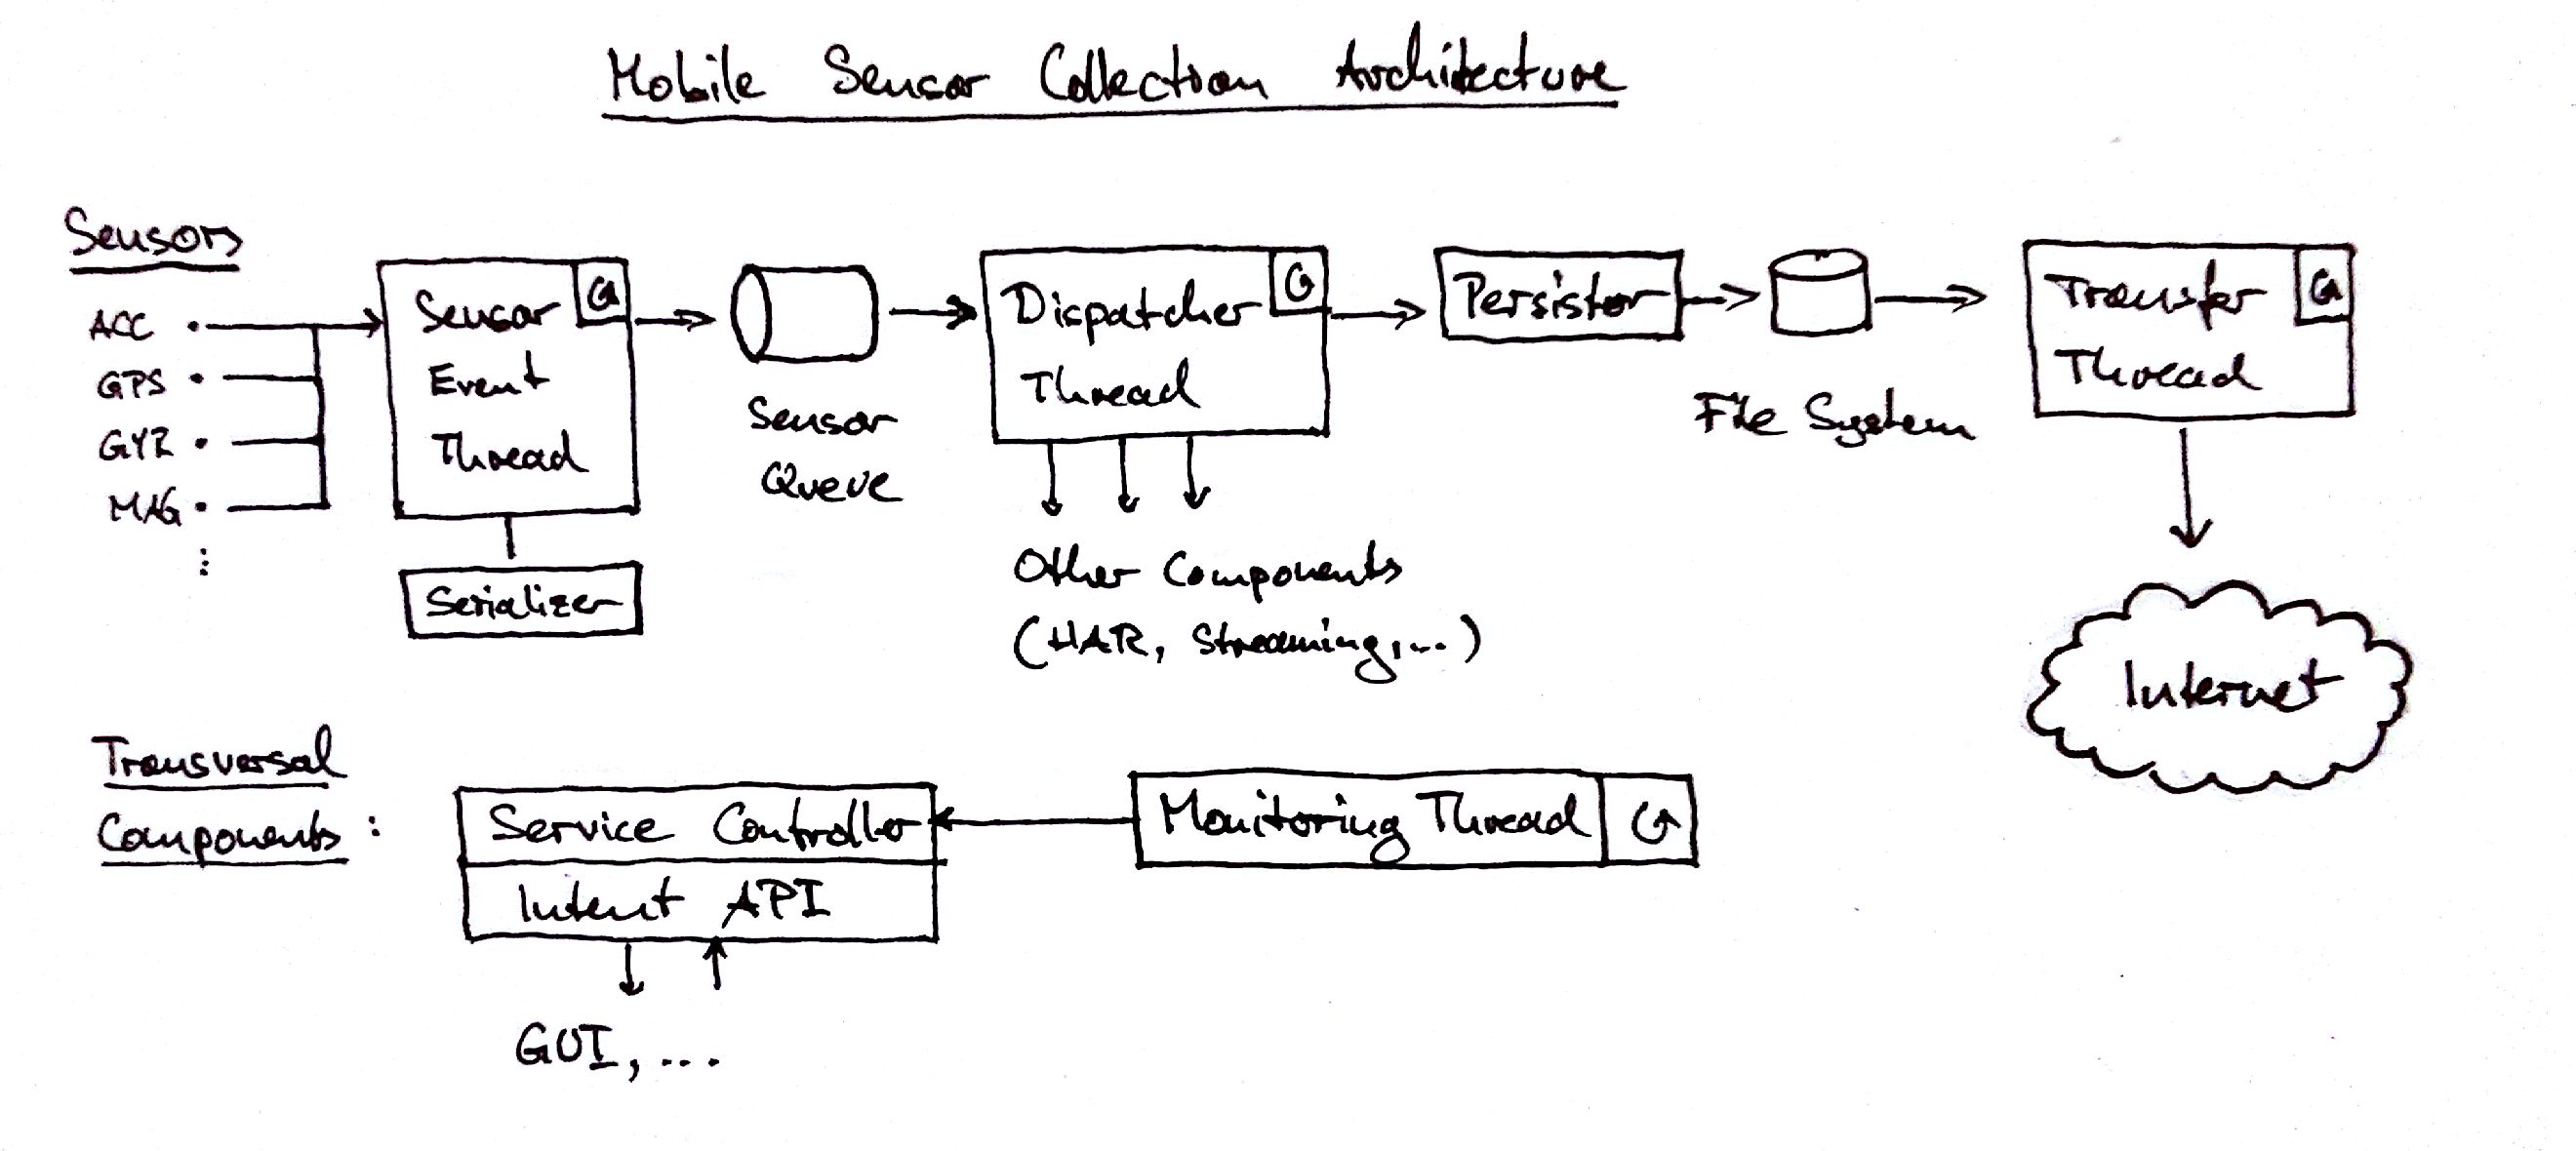
\includegraphics[width=\textwidth]{img/sc/sc_architecture.jpg}
\caption{Sensor Collection Architecture}\label{fig:sc_architecture}
\end{figure}

The architecture consists of the following components:
\begin{itemize}
\item {\bf Sensor Event Thread}. The sensor event thread registers
  callback listeners for all configured sensors. When sensor events
  occur the received values are serialized in the ssf
  format (cf. \ref{sec:ssf}) and pushed onto the SensorQueue.
\item {\bf SensorQueue}. The sensor queue is a synchronized queue
  object that stores sensor values as strings.
\item {\bf DispatcherThread}. The dispatcher thread reads sensor
  values from the sensor queue and passes them to several services
  that can be registered. Included services are the persistor service
  and the activity recognition component, the streaming service and GPS
  publication pipeline (for use in the Service Line Detection API).
\item {\bf Persistor}. The persistor service is executed by the
  DispatcherThread and appends the received sensor sample into a
  predefined file. Also a variant with zip-file compression is
  included.
\item {\bf TransferThread}. The transfer thread is an independent
  thread that transfers the persisted samples to the Live+Gov Servers.
\item {\bf Monitoring Thread}. The monitoring thread polls the
  different components and gathers run-time information like numbers of
  processed samples or transfer state.
\item {\bf Service Controller}. The service controller starts and
  stops all running threads, and takes care of proper configuration of
  all services. It listens to Intents specified in the API and changes
  the state of the service accordingly.
\end{itemize}

The following table summarizes all supported sensors:

\begin{table}[ht]
\centering
\begin{tabular}{|l|p{0.7\linewidth}|}
  \hline
  Sensor & Description \\
  \hline
  GPS                 & Global position in latitude and longitude. 

                        If available, the GPS samples are gathered via
                        Google's new Play Services location
                        provider\footnote{https://developer.android.com/google/play-services/location.html}.
                        The advantages of this library for our use case are: the instant
                        availability of the last known location and a significant decrease
                        of power consumption, since several location providers (e.g. using
                        Wifi) are fused together.  
                        
                        If the Play Services are not available, the service falls back to
                        accessing the GPS samples directly.
  \\ \hline
  Accelerometer       & Measures the acceleration force in $m/s^2$
                        that is applied to a device on all three
                        physical axes. 

                        Also the low-pass and high-pass filtered
                        variants 'Linear Acceleration' and 'Gravity' offered by the Google
                        API can be captured.
  \\ 
  Rotation Vector     & Measures the orientation of a device by
                        providing the three elements of the device's
                        rotation vector.  
  \\
  Gyroscope           & Measures a device's rate of rotation in
                        $rad/s$ around each of the three physical
                        axes. 
  \\ 
  Magnetic field      & Measures the ambient geomagnetic field for all
                        three physical axes in $\mu T$. 
  \\ \hline
  WLAN                & A list of all available wireless local area
                        networks in the transmission range. 
  \\
  Bluetooth           & A list of all available bluetooth clients in
                        the transmission range. 
  \\
  GSM                 & Cellular network operator and the radio cell
                        the mobile phone is connected with. 
  \\ \hline
  Google Activity     & Google recently released an Activity
                        Recognition Library. The sensor collector is able to record activities as sensor
                        values as well. 
  \\
  \hline
\end{tabular}
\caption{Sensors recorded in the Live+Gov sensor collection app}
\label{SensorsOfLGCollectionApp}
\end{table}

\subsection{Intent API}


\label{subsubsec:IntentAPIdescription}

The communication with other Live+Gov toolkit components is
facilitated through the exchange intent
messages\footnote{\url{http://developer.android.com/guide/components/intents-filters.html}}. 
The API was slightly improved since deliverable D1.1. New intents are
marked with an asterisk (*).

The following API-calls are implemented.
\begin{itemize}
\item {\bfseries Start/Stop Service.} Starts and stops the sensor
  collector service. Samples can only be recorded, or transmitted when
  the service is running.
\item {\bfseries Start/Stop Recording.} Starts and stops recording of
  sensor samples.
\item {\bf Send Annotation.} This intent allows users to annotate
  their recording by a string value that will be recorded by a
  ``tag-sensor''.
\item {\bfseries Enable/Disable sample storage.} Samples are stored in
  a local database, of variable size. If Disabled samples can still be
  broadcasted to the system.
\item {\bfseries Enable/Disable continues sample transfer.} Controls
  the sample transfer state machine. When enabled and a network
  connection is available sensor samples are transfered in batches to
  the server backend.
\item {\bfseries Transfer samples.} Triggers the sample transfer.
\item {\bfseries Enable/Disable sample broadcast.} When enabled all
  recorded sensor samples are broadcasted in the form of intents into
  the system. This allows other components, e.g. feature extraction
  and context mining, to make use of the recorded sensor data.
\item {\bfseries Request Status Report.} When this intent is received
  a status report is broadcasted to the system.
\item {\bfseries Tag sample.}  Annotations by users are realized as
  ``Tag sample''.  The content of this intents is included as
  ``tag''-sensor in the recording.
\end{itemize}

When a control intent is received by the component, the appropriate
action is taken. After execution has finished a status report intent
is broadcasted to the system which provides information about whether
the requested method call was successful (cf. Table
\ref{tab:StatusIntent}).  Further technical description of the
component and the API are included in D4.1.

% Status intents contain the following information:
\begin{table}[ht]
\centering
\begin{tabular}{|l|l|l|} \hline
   Key       & Type    & Description                                       \\ \hline
   running   & boolean & True if service is running.                       \\
   recording & boolean & True if sensor samples are recorded.              \\
   storage   & boolean & True if samples are stored in the database.       \\
   transfer  & boolean & True if continues transfer of samples is enabled. \\
   broadcast & boolean & True if samples are broadcasted.                  \\ \hline
\end{tabular}
\caption{Structure of status intents}
\label{tab:StatusIntent}
\end{table}

The sensor sample broadcast intent contains a unique device
identifier, a timestamp and serialized sample data in XML
format. Figure \ref{fig:XMLSamples} shows two examples for GPS and
accelerometer samples.

\subsection{Testing GUI}

\begin{figure}[htbp]
\centering
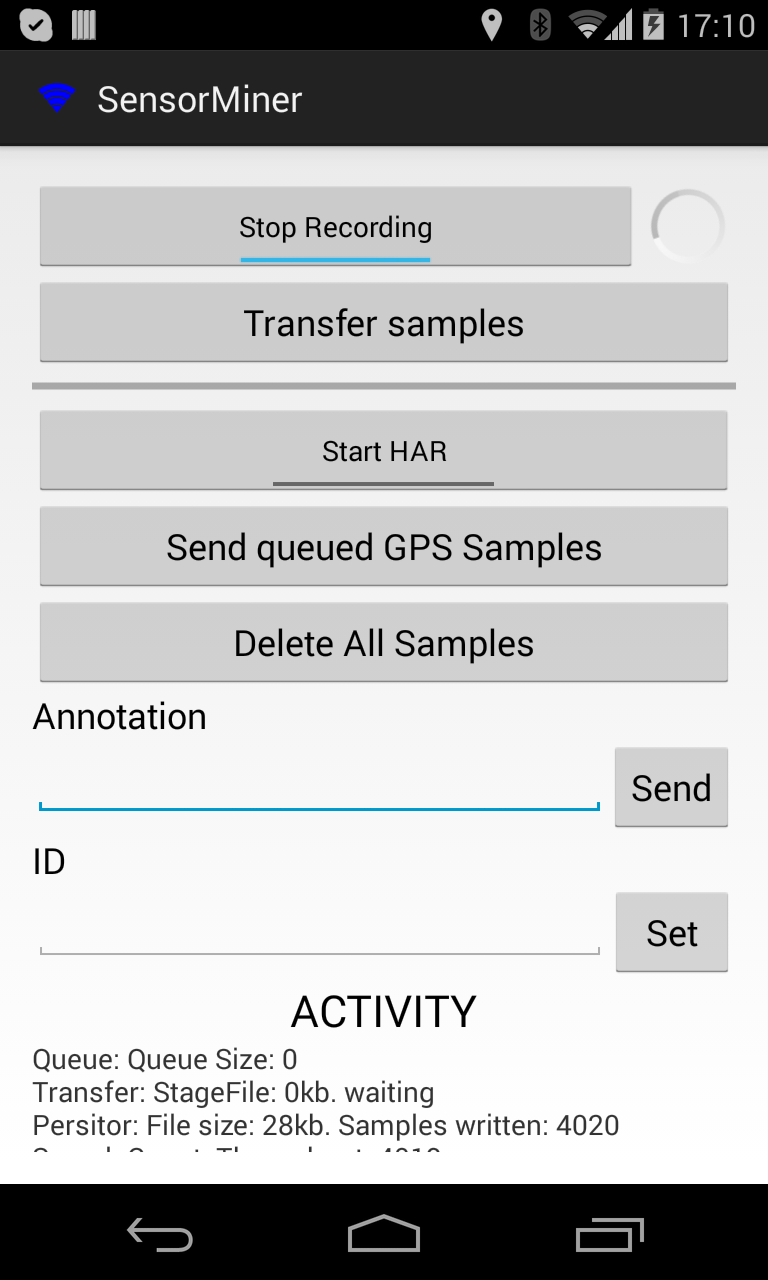
\includegraphics[width=0.3 \textwidth]{img/sc/sc_gui.png}
\caption{Sensor Collection Architecture}\label{fig:sc_gui}
\end{figure}

\subsection{Sensor Stream File Format}\label{sec:ssf}
This document describes the sensor stream format ({\it ssf}) which is used for
transfering sensor values from a mobile device (or another sensor
source) to the Live+Gov data-base. The file format is inspired by the
\href{http://en.wikipedia.org/wiki/Common\_Log\_Format}{Common Log
  Format} used by many webservers. We view incoming sensor values as
events and record them as a simple stream of CSV-rows. Each sensor has
an individual prefix but writes into the same file.

The key advantages of this format as opposed to the previously used
XML format are:
\begin{itemize}
\item Human readability. The format is easy to understand by humans.
\item Statelessness. Every line can be interpreted without the context
  of the file. Therefore ssf-files can be arbitrarily sliced,
  concatenated and filtered using UNIX tools like {\it grep, cat, sed,
    awk}.
\item Streaming. Lines can be individually transferred over tcp
  sockets or messaging systems. Allowing immediate inspection of the
  recorded samples on a remote system.
\end{itemize}

\subsubsection*{Format Description}

The rows of the ssf-format have the following structure:
\small
\begin{verbatim}
SENSOR_PREFIX,TIME_STAMP, USER_ID, SENSOR_VALUES
\end{verbatim}
\normalsize


The authorative source for the field descriptions is the source code.

\begin{itemize}
\item \texttt{SENSOR PREFIX}. Identifies the sensor producing the
  sample. The following sensor prefixes are supported: \\
  \texttt{GPS} (GPS sensor), \texttt{ACC} (Accelerometer),
  \texttt{LAC} (Linear Acceleration), \texttt{GRA} (Gravity),
  \texttt{GYR} (Gyroscope), \texttt{MAG} (Magnetometer), \texttt{WIFI}
  (Wifi networks), \texttt{BLT} (Bluetooth), \texttt{GSM} (GSM cells),
  \texttt{ACT} (Google Play Services Activity), \texttt{ERR} (Error
  Value), \texttt{TAG} (Annotations entered by the user).
\item \texttt{TIME STAMP} UNIX timestamp in milliseconds e.g. \texttt{1377609577214}
\item \texttt{USER ID} ID that identifies records from the same
  user. The default value is the device-id that is provided by
  Android.
\item \texttt{SENSOR VALUES} 
  Sensor values in individual formats. In order to adhere to the CSV
  standard no \texttt{,}-symbol and new-lines may be used in this field.
  \begin{itemize}
  \item \texttt{ACC/GYR/MAG/LAC/GRA} X,Y,Z-values separated by space characters.
  \item \texttt{GPS} lat,lon,alt-values separated by space characters
  \item \texttt{ACT} Activity Name, Confidence separated by space characters.
  \item \texttt{WIFI} List of access-points, where each visible
    accesspoint is separated by a \texttt{;} and written as

    Escaped SSID String/Escaped BSSID String/Frequency in MHz/RSSI in dBm
  \item \texttt{BLT}
    List of devices where each visible device is separated by a \texttt{;}
    and written as
    Escaped Address/Device Major Class/Device Class/Bond
    State/Optional Escaped Name/Optional RSSI
  \item \texttt{GSM}
    The state of the device written as Service State/Roaming State/Manual
    Carrier Selection State/Escaped Carrier Name/Escaped Signal Strength

    followed by \texttt{:}, followed by a possibly empty list of cells,
    where each cell is separated by a \texttt{;} and written as
    Escaped Cell Identity/Cell Type/RSSI in dBm
  \end{itemize}
\end{itemize}

Example rows may look as follows:
\small
\begin{verbatim}
ACC,1377605748123,5,0.9813749 0.0021324 0.0142523
GPS,1377605748156,5,50.32124 25.2453 136.5335
WIFI,1341244415,wifiUser,"WiFi AP"/"00:12:42"/2412/-45; "Another WiFi AP"/"33:13:53"/2437/-56
TAG,1378114981049,anotherUser,"test tag"
BLT,1385988380374,bluetoothUser,"C8:F7:33:B7:B5:B4"/computer/computer laptop/bonded/"LAPTOP"/-46
\end{verbatim}
\normalsize

\subsection{Streaming Service}

The revised version of the sensor collector includes a streaming
service, that transfers recorded samples directly to a remote machine.

The streaming service uses the ZeroMQ networking
library\footnote{http://www.zeromq.org} to transfer single ssf lines
to the Live+Gov machine running a streaming server. The streaming
server appends the received samples to a file (zmq\_stream.ssf).

This simple service allows direct monitoring of the recorded samples,
via simple UNIX command line tools, e.g. 
\begin{verbatim} 
tail -f zmq_stream.ssf 
\end{verbatim}
prints the recoded samples to the console.
\begin{verbatim} 
tail -f zmq_stream.ssf | grep ^GPS 
\end{verbatim} 
filters out gps samples. And finally
\begin{verbatim} 
tail -f zmq_stream.ssh | cut --delimiter=',' --field=1 | logtop  
\end{verbatim}

shows the frequencies of the individual incoming sensor values.

\section{Sensor Storage Service Architecture}

\begin{figure}[htbp]
\centering
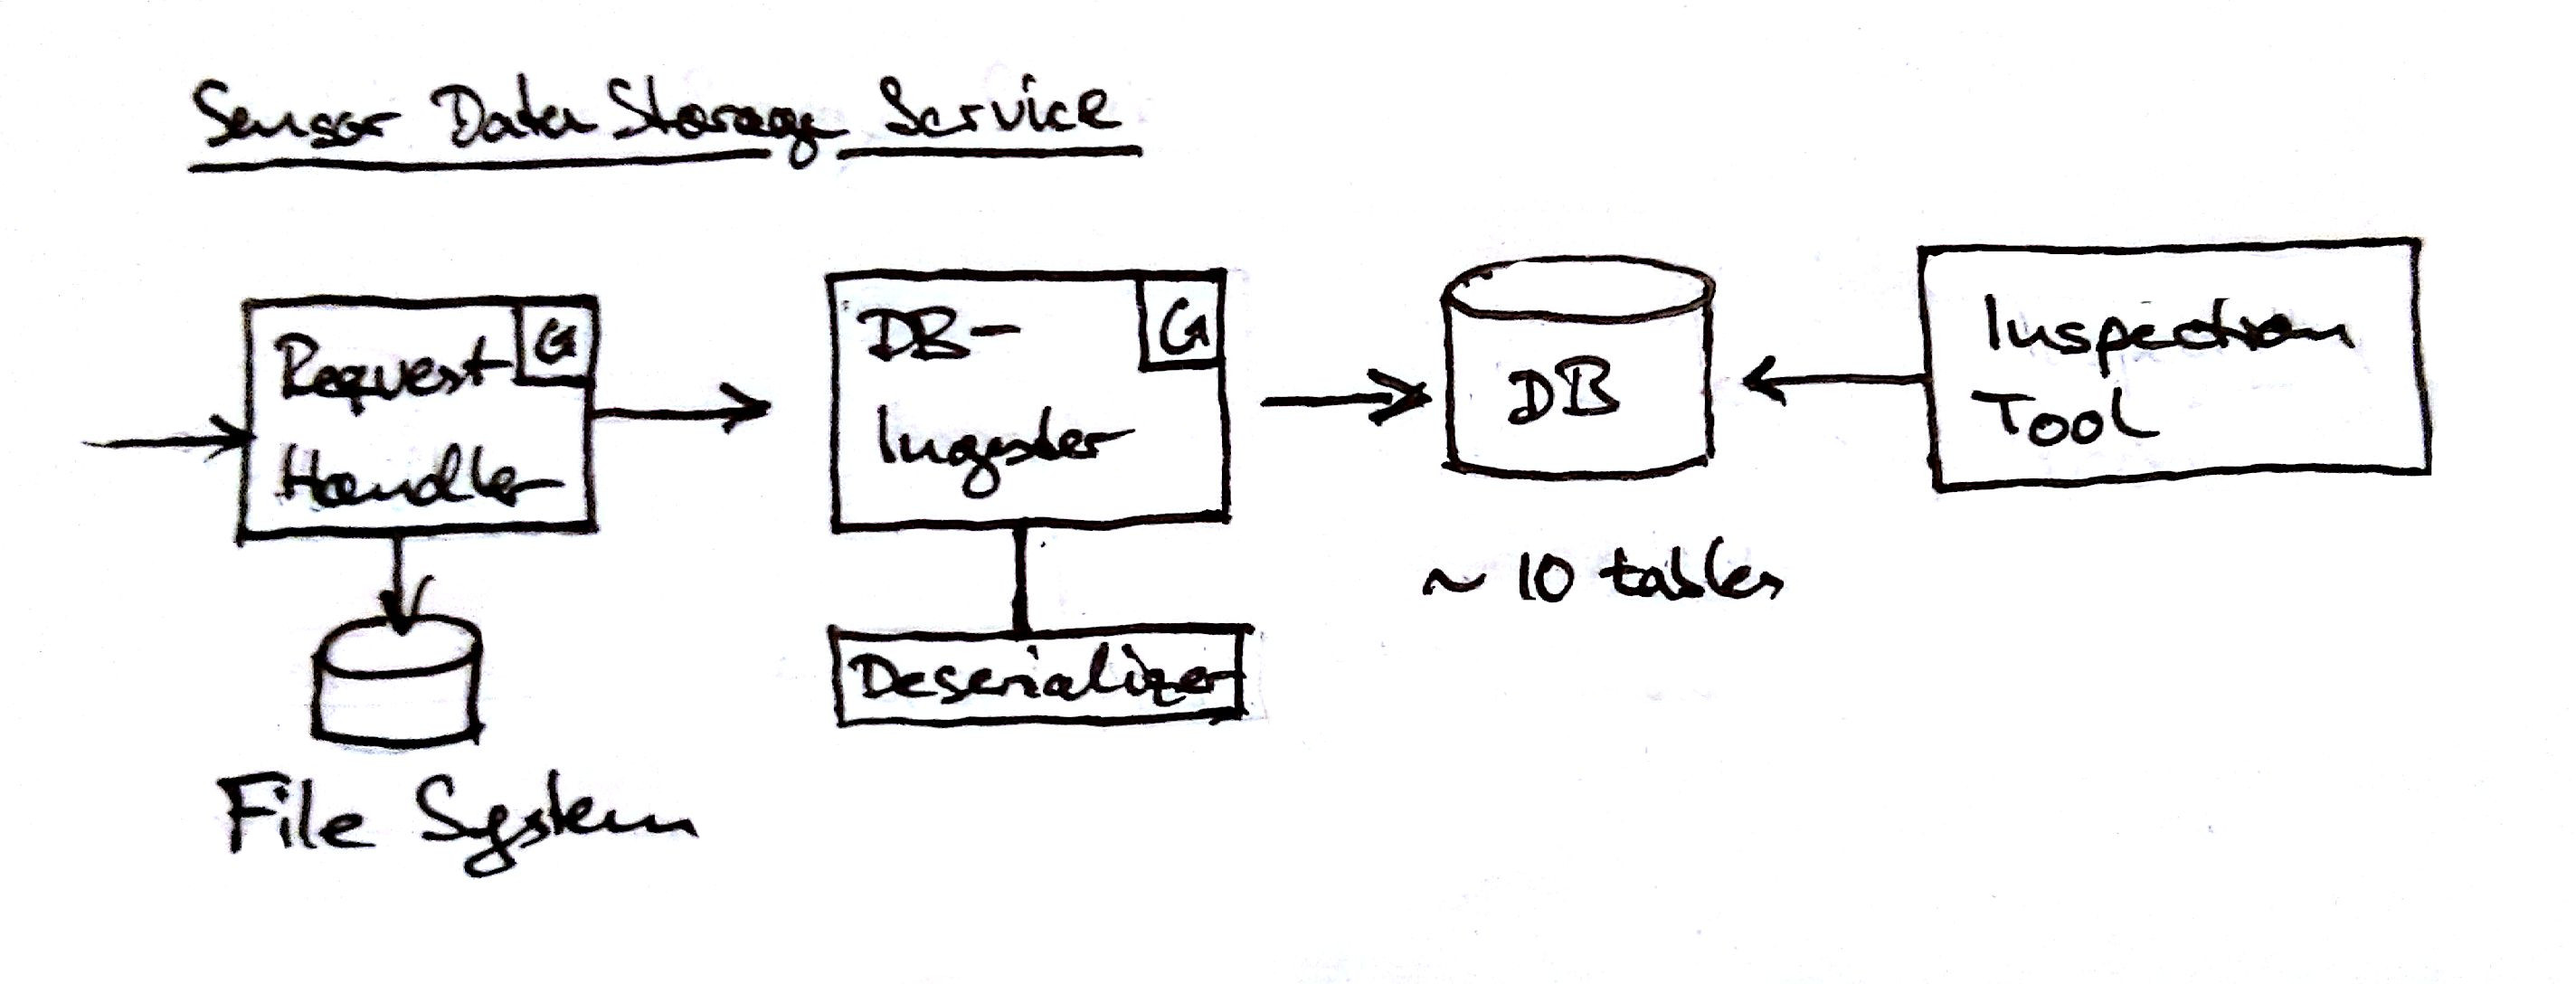
\includegraphics[width=0.7\textwidth]{img/sc/ss_architecture.jpg}
\caption{Sensor Collection Architecture}\label{fig:ss_architecture}
\end{figure}

Architecture Description

\subsection{Database Scheme}

The uploaded samples are stored in a
PostgreSQL\footnote{http://www.postgresql.org/} database. We have
switched from MySQL to this technology, because of the advanced query
fuctionality that is offered by the
PostGIS\footnote{http://postgis.net/} plugin.

The database has the following schema:
{\small
\begin{verbatim}
sensor_gps (trip_id INT, ts BIGINT, lonlat GEOGRAPHY(Point));
sensor_accelerometer (trip_id INT, ts BIGINT, x FLOAT, y FLOAT, z FLOAT);
sensor_linear_acceleration (trip_id INT, ts BIGINT, x FLOAT, y FLOAT, z FLOAT);
sensor_gravity (trip_id INT, ts BIGINT, x FLOAT, y FLOAT, z FLOAT);
sensor_tags (trip_id INT, ts BIGINT, tag TEXT);
sensor_google_activity (trip_id INT, ts BIGINT, activity TEXT);
har_annotation (trip_id INT, ts BIGINT, tag TEXT);
\end{verbatim}}

\subsection{Inspection Front End}


\subsection{Integration of Logging and Heartbeats}



\subsection{Cross-Platform Strategy}
Explain problems with Titanium framework.

Android component runs on Blackberry. 

Implement HAR as SAAS. Write client app for iOS.


%%% Local Variables:
%%% mode: latex
%%% TeX-master: "../D1-2"
%%% End:


\chapter{Reality Mining Methods}

\section{Human Activity Recognition}
%%%%%%%%%%%%%%%%%%%%%%%%%%%%%%%%%%%%%%%%%%%%%%%%%%%%%%
%\section{Human Activity Recognition}
%%%%%%%%%%%%%%%%%%%%%%%%%%%%%%%%%%%%%%%%%%%%%%%%%%%%%%
\label{sec:HAR}

\newcommand{\IR}{\mathbb{R}}

In this section we describe the implementation of the human activity
recognition ('HAR') component on the mobile device.  The algorithmic
foundations of this data mining task have been described in detail in
deliverable D2.2 in section 3.2 ``Mobile Sensing and activity
recognition''. We include a brief summary here (\ref{sec:har_method})
for the sake of completeness. Subsection \ref{sec:har_component}
contains the descriptions of the implementation. In subsection
\ref{sec:har_eval} we evaluate our method on two data sets and compare
it to the state of the art approaches.

\subsection{HAR Method Summary}\label{sec:har_method}

The process of activity recognition uses a pipeline of signal
processing and machine learning techniques. It consists of two phases:
the ``training phase'' and the ``integration phase''. 

\begin{figure}[htbp]
\centering
\subfigure[HAR Training Phase]{
\label{fig:har_overview}
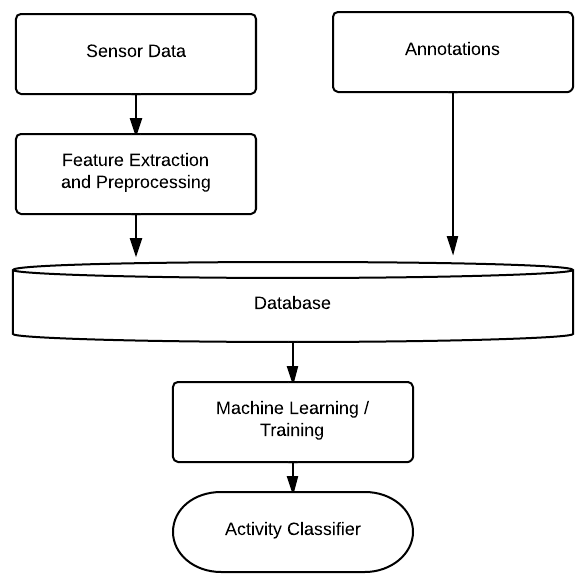
\includegraphics[width=0.45 \textwidth]{img/har/classification_overview.png}
} \hspace{1cm}
\subfigure[HAR Integration Phase]{
\label{fig:integrated_har_overview}
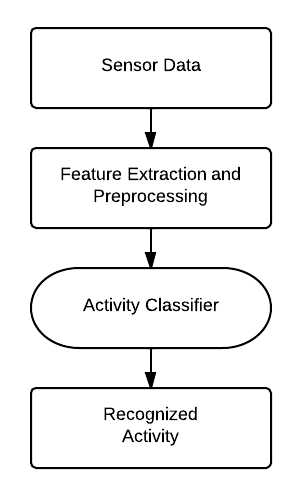
\includegraphics[width=0.25 \textwidth]{img/har/integration_overview.png}
}
\caption{Human Activity Recognition Method Overview}
\label{fig:HAR_PHASES}
\end{figure}

In the training phase (cf. Figure \ref{fig:har_overview}) a group of
volunteers is asked to perform the targeted activities for a certain
amount of time, while recording sensor samples with the device in
their pocket.  The gained training data stored in a database and used
to train a classifier of the activities.

In the integration phase (cf. \ref{fig:integrated_har_overview}), the
trained classifier is embedded into the mobile device.

Both phases rely on the preprocessing steps of "windowing'' and
``feature generation''. The stream of incoming sensor data is divided into
time windows of fixed size (typically 1-10 sec.) and for each window
a set of features is computed. This features are filtering out
relevant information from the raw signal. Typical features include
mean values and standard deviations as well as frequency domain
features like Fourier modes.

Deliverable D2.2 contains detailed lists of all sensors and features
and data mining methods that are used in the literature as well as
discussions of quality of the recognition results.

\subsection{Component Description}\label{sec:har_component}

The Human Activity Recognition Component implements the two phases
described in Figure \ref{fig:HAR_PHASES}. The training phase is
executed offline on a server and uses the following processing
pipeline (cf. Figure \ref{fig:classification_architecture}).

\begin{figure}[htbp]
\centering
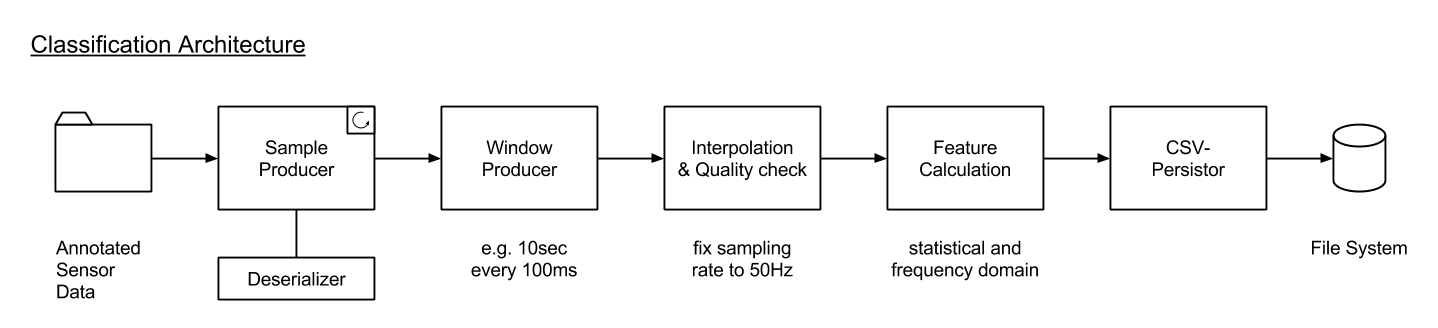
\includegraphics[width=\textwidth]{img/har/classification_architecture.png}
\caption{HAR Training Pipeline}\label{fig:classification_architecture}
\end{figure}

\begin{enumerate}
  \item {\bf Annotated Sensor Data.} The training data is stored as
    ssf files in the file system. The annotations are represented as
    folder structure. In this way it becomes very easy to add new
    training data to the repository. Using the inspection web tool,
    one can select appropriate time slices and export the
    corresponding samples as ``.ssf'' file. The exported file is then
    moved to the folder corresponding to the recorded activity.
  \item {\bf Sample Producer.} The sample producer service reads the 
    sensor samples from the file system and pushes them onto a generic 
    sample processing pipeline. The interface is designed a way that
    resembles the incoming data stream on the mobile device.
  \item {\bf Window Producer.} The window producer takes as
    constructor parameters a window-length and a delay. Incoming
    sensor samples are grouped in windows of the given length and
    passed further down as a single object.
  \item {\bf Interpolation and Quality Check.}  
    The recorded sensor data can be subject so several irregularities,
    like frequency disparities or small outtakes. To ensure that those
    irregularities do not pollute the training data we perform quality
    checks on the individual windows and interpolate the samples to a
    constant frequency of $50Hz$.
  \item {\bf Feature Calculation.} The classification calculates
    different features extracted from windows of raw sampling data. A
    description of the used features is included in section
    \ref{sec:feature_calc}.
  \item {\bf CSV-Persistor.} The calculated feature vectors are stored
    on the file system as CSV file. 
\end{enumerate}

In the next step the stored annotated feature vectors are used for
training of machine learning classifiers. For this task we relyed on 
available external tools like
WEKA\footnote{\url{http://www.cs.waikato.ac.nz/ml/weka/}}
and libsvm\footnote{\url{http://www.csie.ntu.edu.tw/~cjlin/libsvm/}}.
More details of the classification methods are given in section
\ref{sec:har_classifier_training}.
The trained classifiers were then exported as java methods and
integrated into the mobile HAR service (cf. Figure \ref{fig:integrated_har}).

\begin{figure}[htbp]
\centering
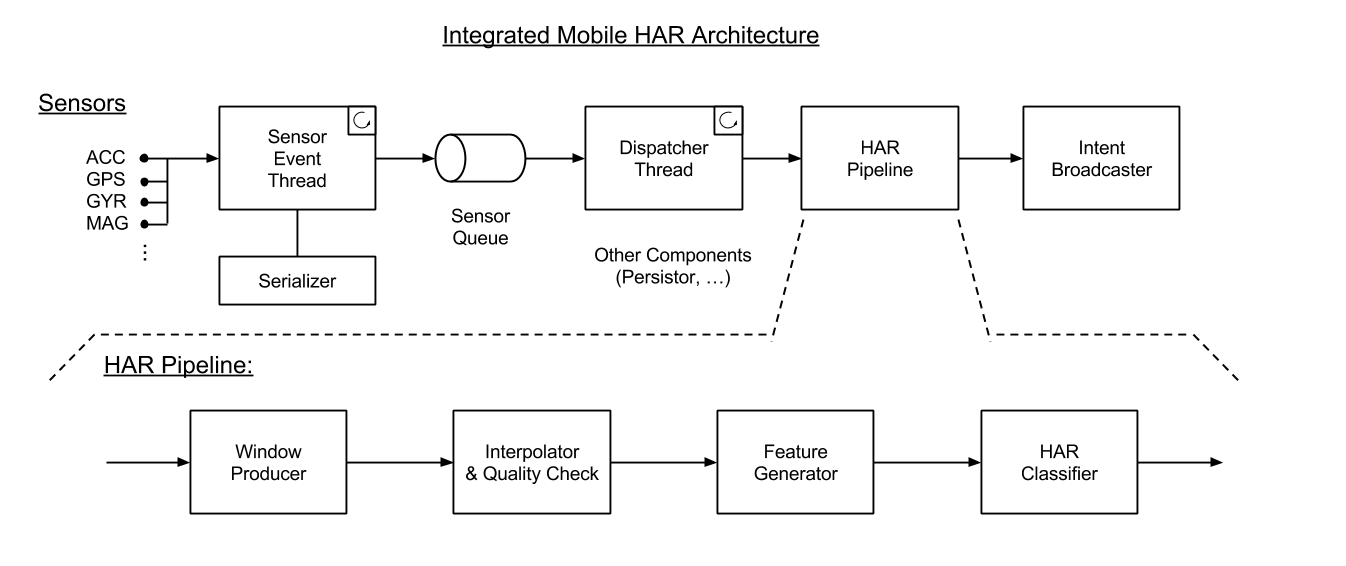
\includegraphics[width=\textwidth]{img/har/integration.png}
\caption{Integrated HAR Architecture}\label{fig:integrated_har}
\end{figure}

The integrated mobile HAR architecture consists of the following components.
\begin{enumerate}
\item {\bf Dispatcher Thread.} The dispatcher thread is part of
  the sensor collection architecture described in Chapter
  \ref{chap:sc}. It emits all gathered samples in the ssf format.
\item {\bf HAR Pipeline.} The HAR pipeline reuses most parts described
  in Figure \ref{fig:classification_architecture}. The Sample Producer
  is replaced by the Dispatcher Thread as source for sensor data.
\item {\bf HAR Classifier.} The HAR classifier component warps
  exported java method and outputs the results of the classification
  as string objects. The current implementation uses a decision tree.
\item {\bf Intent Broadcaster.} The classification results are
  broadcasted as an intent for use in other parts of the system
  (e.g. GUI, storage).
\end{enumerate}

\subsection{Feature Calculation}
\label{sec:feature_calc}

For the classifiaction of activities, we cannot directly use the raw
stream of sensor data. The reason is that machine learning classifiers
cannot operate on data streams directly, but need to get explicit
vectors as input. Moreover, these vectors cannot have arbitrary
dimension. If we feed in the raw sensor signal of only 5 seconds
recording, we get a vector of dimension
\[ d = 50 Hz \cdot 5 sec \cdot 3\ axes = 1000, \]
which is too much to handle for most classification algorithms.

With the calculation of features, we try to reduce the dimensionality
of the input signal, while keeping the essential information contained
in the signal. We use two different methods for feature calculation
{\it manual selection} and an automated {\it PCA} based feature set.

\subsubsection*{\bf Manually Selected Features}

The following manual features have been selected:

\begin{center}
\begin{tabular}{|r|l|p{11.5cm}|} \hline
Index & Name     & Description \\ \hline
0            & id       & User ID of the recorded samples \\ \hline
1            & tag      & Name of the recoded activity    \\ \hline
2            & xMean    & Mean values of the individual axes \\ 
3            & yMean    &             \\ 
4            & zMean    &             \\ \hline
5            & xVar     & Variance of the individual axes  \\ 
6            & yVar     &             \\ 
7            & zVar     &             \\ \hline
8            & s2Mean   & Mean value of the length of the acceleration
                          vector. \\ \hline
9            & s2Var    & Variance of the length of the acceleration
                          vector \\ \hline
10           & tilt     & Average tilting angle of the device towards
                          the vertical axes. \\ \hline
11           & energy   & Total energy of the recording.  \\ \hline
12           & kurtosis & Kurtosis\footnote{\url{http://en.wikipedia.org/wiki/Kurtosis}} 
                          measure of "peakedness" of the length of 
                          the acceleration vector. \\ \hline
13-24        & S2Bins   & Histogram over the length of the
                          acceleration vector. \\ \hline
25-37        & FFTBins  & Historgram over the absolute values of the
                          Fourier Modes of the length of the
                          acceleration vector. \\ \hline
\end{tabular}
\end{center}

Our feature list has been guided by the literature (cf. D1.2,
\cite{lara12}).  These consist of statistical features (mean and
variance), that are computed for each of the three axes as well as for
the length of the acceleration vector $s_2 = \sqrt{x^2 + y^2 + z^2}$.
An explicit tilt-feature has been included to allow better separation
of the ``sitting'' and ``standing'' classes.

We also include frequency domain features.  The ``energy'' feature
measures the total spectral
density\footnote{\url{http://en.wikipedia.org/wiki/Spectral_density}}
of the signal. Furthermore a set of histogram features measures the
energy of different Fourier modes of the signal. We have divided
energy spectrum into 10 equally distributed bins, covering roughly
95\% of the observed energy spectrum in the training data. Two more
bins added for outliers above and below the bin coverage.

\subsubsection*{\bf PCA Based Features}

There is a lot of freedom in the manual choice of feature vectors.
Moreover, it is not clear that the heuristically selected features
are able to separate the categories well. An automated way of
selecting features is provided by the {\it Principal Component
  Analysis} (PCA) method.\footnote{\url{http://en.wikipedia.org/wiki/Principal_component_analysis}}
This method selects a number of linear features that maximize 
variance of the resulting data. We use a reduced vector size of $266$
dimensions to keep $90\%$ of the variance in our data set.

\subsection{Classifier Training}\label{sec:har_classifier_training}

In this section we present more details about the employed machine
learning methods for human activity recognition. Both methods rely on
a training set of annotated feature vectors, and cannot be used
directly on the data-streams. As was explained in D2.1 the two
presented methods are the most popular approaches in the literature
and have led to good classification accuracies in earlier work.

\subsubsection*{{\bf Decision Tree HAR classifier}}
\label{sec:DectionTree}

A decision tree uses a hierarchy of simple binary decisions to
classify a feature vector into a set of given categories.  To be more
precise, let $x_\bullet = (x_1, \dots, x_n)$ a feature vector with numeric
feature values $x_i \in \IR$, and $C=\{c_1, \dots, c_N\}$ a set of
target categories. The individual decision rules $R_k$ are of the form
$(x_j \geq \alpha)$ or $(x_j \leq \alpha)$ for some index $j$ and
threshold value $\alpha \in \IR$.  A decision tree, organizes several
of those rules $R_k$ into a binary tree structure. The leaf nodes are
linked to the corresponding target categories. Figure
\ref{fig:decision_tree} shows an example of a tree with 9 decision
nodes and 4 categories.

\begin{figure}[h]
\centering
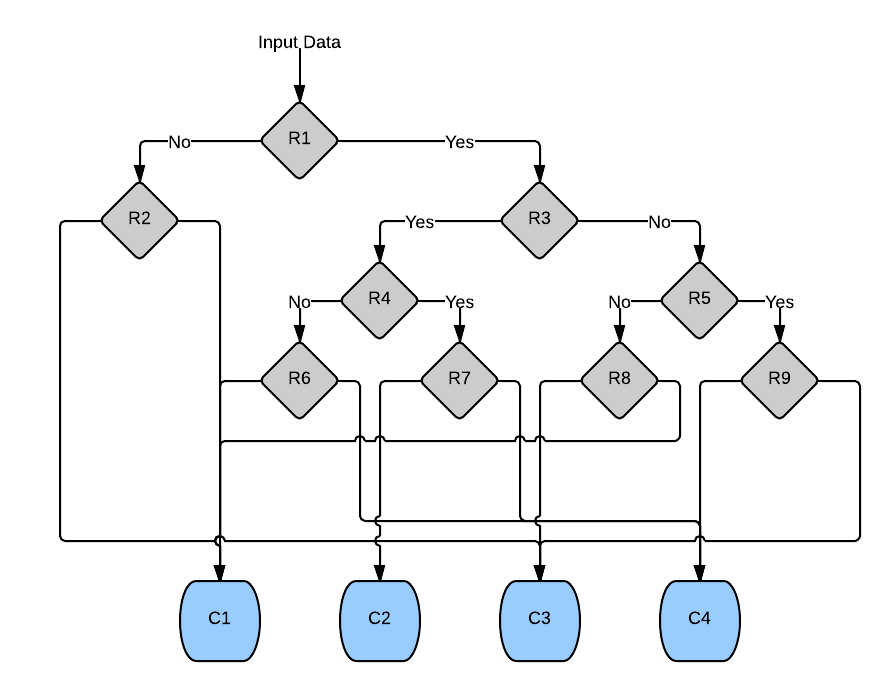
\includegraphics[width=0.5 \textwidth]{img/har/decision_tree.png}
\label{fig:decision_tree}
\caption{An example of a decision tree.}
\end{figure}

In the case of the activity recognition classifier, we have the
different activities (e.g. standing, walking, running) as 
categories and a set of manually computed features like (standard
deviations, or bin distributions of Fourier-modes) or automatically
generated PCA-based features to base our decision rules on.

Of course, we do not want to build a decision tree for the HAR task by
hand, but automatically learn a suitable tree on the basis of
annotated training data. For this task of decision tree learning,
several methods are known. Notable ones
include\footnote{\url{http://en.wikipedia.org/wiki/Decision_tree_learning}}:
ID3 (Iterative Dichotomiser 3), C4.5 (successor of ID3), CART
(Classification And Regression Tree), CHAID (CHi-squared Automatic
Interaction Detector).

We have chosen to use the C4.5 algorithm modified for continues
attribute values \cite{quinlan1996improved} since it has been
successfully used in the literature \cite{lara12} and an open source
implementation is available and integrated into the WEKA toolkit.

The C4.5 algorithm uses the concept of {\it information gain} to build
up a decision tree in a recursive, greedy fashion.  For a set of
annotated training vectors $T = \{ (x_\bullet, c) | c \in C \}$ a
decision rule $R$ splits $T$ into two subsets:
\[ T = T^+ \cup T^{-}, \quad T^+ = \{ R(x_\bullet, c) = \text{true}\}, \;
T^- = \{ R(x_\bullet, c) = \text{false} \} \]
The information gain of this rule is defined as 
\[ IG(T,R) = H(T) - \frac{|T^+|}{|T|} \cdot H(T^+) - \frac{|T^-|}{|T|} \cdot H(T^-), \]
where $H(S)$ is the entropy of the collection $S \subset T$
cf. \cite{Shannon1948}. The C4.5 algorithm finds the decision rule
with the largest information gain and uses this as the root for the
decision tree. It then recurses into the subset $T^+$ and $T^-$ and
adds the generated nodes as childs to the root node.

The choice of the threshold values $\alpha$ for the decision rules is
particularly crucial for the quality of the trained decision tee. A
possible improvement of the threshold selection algorithm can be
obtained by pre-clustering of the attribute values before the
training process cf. \cite{kotsiantis2006}.

Figure \ref{fig:dt_example} shows an example of a trained decision
tree on manually generated features.

\begin{figure}[h]
\tiny
\centering
\begin{verbatim}
J48 pruned tree
------------------

Number of Leaves  : 	52

Size of the tree : 	103


x18 <= 927
|   x24 <= 152
|   |   x20 <= 211
|   |   |   x4 <= -2.936108
|   |   |   |   x3 <= 1.132095
|   |   |   |   |   x18 <= 458
|   |   |   |   |   |   x35 <= 2: WALKING (6.0/1.0)
|   |   |   |   |   |   x35 > 2: CYCLING (2.0)
|   |   |   |   |   x18 > 458: SITTING (3.0)
|   |   |   |   x3 > 1.132095: CYCLING (527.0)
|   |   |   x4 > -2.936108
|   |   |   |   x4 <= 7.830095
|   |   |   |   |   x14 <= 13
|   |   |   |   |   |   x18 <= 87
|   |   |   |   |   |   |   x2 <= 3.434441
|   |   |   |   |   |   |   |   x3 <= -2.172633
|   |   |   |   |   |   |   |   |   x2 <= -3.51528: RUNNING (3.0/1.0)
|   |   |   |   |   |   |   |   |   x2 > -3.51528: WALKING (45.0/1.0)
|   |   |   |   |   |   |   |   x3 > -2.172633: CYCLING (5.0/1.0)
|   |   |   |   |   |   |   x2 > 3.434441
|   |   |   |   |   |   |   |   x19 <= 469: CYCLING (155.0)
|   |   |   |   |   |   |   |   x19 > 469: WALKING (4.0/1.0)
|   |   |   |   |   |   x18 > 87
|   |   |   |   |   |   |   x18 <= 415
|   |   |   |   |   |   |   |   x15 <= 17
|   |   |   |   |   |   |   |   |   x34 <= 60
|   |   |   |   |   |   |   |   |   |   x22 <= 138
|   |   |   |   |   |   |   |   |   |   |   x20 <= 98
|   |   |   |   |   |   |   |   |   |   |   |   x21 <= 58: CYCLING (10.0)
|   |   |   |   |   |   |   |   |   |   |   |   x21 > 58: WALKING (56.0)
|   |   |   |   |   |   |   |   |   |   |   x20 > 98
|   |   |   |   |   |   |   |   |   |   |   |   x17 <= 108

// TRUNCATED

x18 > 927
|   x10 <= 0.58851: SITTING (1071.0)
|   x10 > 0.58851
|   |   x3 <= -8.323328: WALKING (17.0)
|   |   x3 > -8.323328: CYCLING (15.0/2.0)
\end{verbatim}
\normalsize
\caption{Decision tree trained on manually computed features.}
\label{fig:dt_example}
\end{figure}

\subsubsection*{{\bf Support Vector Machine HAR Classifier}}
\label{sec:SVM}

A popular algorithm to train a binary classification model for mapping
features to activities is the Support Vector Machines (SVMs). SVMs are
known for their ability in smoothly generalizing and coping
efficiently with high-dimensionality pattern recognition
problems. They define a hypothesis space that includes all the
possible linear separations of the data
(Fig.~\ref{fig:svm_hypothesisSpace}) and they choose the one that
maximizes the margin between the two classes
(Fig.~\ref{fig:svm_margin}).

\begin{figure}[h]
\centering
  \includegraphics[width=0.5\textwidth]{img/svms/Svms_hypothesisSpace.pdf}
  \caption[Hypothesis spaces for SVM classifier.]{Left: Hypothesis space including all linear separations. Right: The selected hypothesis maximizes the margin.}
  \label{fig:svm_hypothesisSpace}
\end{figure}


\begin{figure}[h]
\centering
  \includegraphics[width=0.5\textwidth]{img/svms/Svm_Maxmargin.pdf}
  \caption{Maximization of the margin}
  \label{fig:svm_margin}
\end{figure}

\noindent The hyperplane that optimally separates the positive and the
negative class (i.e. maximizes the margin) can be described by
$\mathbf{w\cdot x + b = 0}$, where $\mathbf{w}$ is normal to the
hyperplane and $\frac{b}{\parallel\mathbf{w}\parallel}$ is the
perpendicular distance from the hyperplane to the origin
(Fig.~\ref{fig:svm_wb}). The optimal hyperplane can be obtained by
solving the following Quadratic Programming optimization problem:

\begin{equation}\label{Eq:svmQP0}
  \min \frac{1}{2}\parallel\mathbf{w}\parallel \quad \text{s.t.} \quad y_i(\mathbf{w}\cdot x_i + b) -1 \ge 0 \quad \forall i
\end{equation}

In order to relax the constraints of Eq.~\ref{Eq:svmQP0} and allow for
some misclassified points, a slack variable $\xi_i, i=1,\ldots,L$ is
introduced which transforms Eq.~\ref{Eq:svmQP0} into:

\begin{equation}\label{Eq:svmQPxi}
  \min \frac{1}{2}\parallel\mathbf{w}\parallel + C\sum_{i=1}^{L}\xi_i \quad \text{s.t.} \quad y_i(\mathbf{w}\cdot x_i + b) -1 +\xi_i \ge 0 \quad \forall i
\end{equation}

\noindent where the parameter $C$ controls the trade-off between the
slack variable penalty and the size of the margin. In the testing
phase, in order to classify an unseen example $x_t$, its distance to
the hyperplane is calculated using the formula $\mathbf{w}\cdot x_t +
b$. This distance indicates the classifier's confidence that the
unseen example $x_t$ belongs to the examined class.

\begin{figure}[h]
\centering
  \includegraphics[width=0.6\textwidth]{img/svms/Svms_wb.pdf}
  \caption{The resulting hyperplane after training an SVM.}
  \label{fig:svm_wb}
\end{figure}

The previous consider linear separation of the data. However, this is
rarely the case for most real world scenarios and for this reason the
kernel trick has been introduced. Applying the kernel trick to the
cases where the classes are not linearly separable in the input
feature space, we manage to map the features to a higher dimension
(Fig.~\ref{fig:svm_highDim}) where they can be linearly separated. For
example, in the case of an RBF kernel the otherwise linear hyperplane
is transformed to a hypersphere (Fig.~\ref{fig:svm_rbf}). For any
kernel $K(x,y)$, the classification model can be represented by a
vector $\textbf{w}$ (i.e. the model parameters), a bias scalar $b$ and
the support vectors $\mathbf{SV}_j, j=1,\ldots,N_{SV}$. For an unseen
example $x_t$, a confidence score is extracted by computing its
distance to the hyperplane of the model:

\begin{equation}\label{Eq:SVMdecision}
  confidence = \mathbf{w}*\sum_{j=1}^{N_{SV}}{K(\mathbf{SV}_j,\mathbf{x}_t)}+b
\end{equation}

\begin{figure}[h]
\centering
  \includegraphics[width=0.6\textwidth]{img/svms/Svm_DimensionMap.pdf}
  \caption{Illustration of the kernel trick for sample separation.}
  \label{fig:svm_highDim}
\end{figure}

\begin{figure}[h]
\centering
  \includegraphics[width=0.6\textwidth]{img/svms/Svm_RBF.pdf}
  \caption{Non-linear separation of the data using the RBF kernel}
  \label{fig:svm_rbf}
\end{figure}


In our case, an SVM model is trained on the previously extracted
features in order to learn the properties that define the examined
activity. The models are trained using the one versus all (OVA)
technique, i.e. all positive examples of the specific activity versus
all negative examples (i.e. the examples of all other activities). The
distance of a vector from the hyperplane indicates our confidence that
during the analysed window, the user performs the examined
activity. High positive values of this score increase our confidence
that this window belongs to the positive class while high negative
values provide strong confidence that the performed activity is not
the examined one.

% The fact that each model can be represented by a single vector and a
% scalar and that the testing process is essentially a vector
% multiplication, renders SVMs the best solution for a real time
% classification framework. This allows for storing the information
% about all the models in the phone memory, while testing is
% computationally very efficient, making it possible for the image
% classification algorithm to run entirely on a mobile phone.


\subsection{Evaluation}\label{sec:har_eval}

We have evaluated our classifier on two different datasets.

The first dataset was gathered on the University Campus in Koblenz in
December 2013.  It contains a total of around $900K$ samples collected
by $10$ volunteers.  The volunteers were instructed to perform the
activities ''walking'', ''running'', ''stairs'' and ''cycling'' on
predefined routes on the university campus. 
% (cf. Figure \ref{fig:data_collection_handout}). 
The total time effort per volunteer was about 20-25minutes and a financial reward was offered as
an incentive. After the recording the samples have been inspected
using our inspection tool and the beginning and ending of the
activities were manually stripped in order to avoid noise from holding
the device in the hand.

% \begin{figure}[htbp]
%   \centering
%   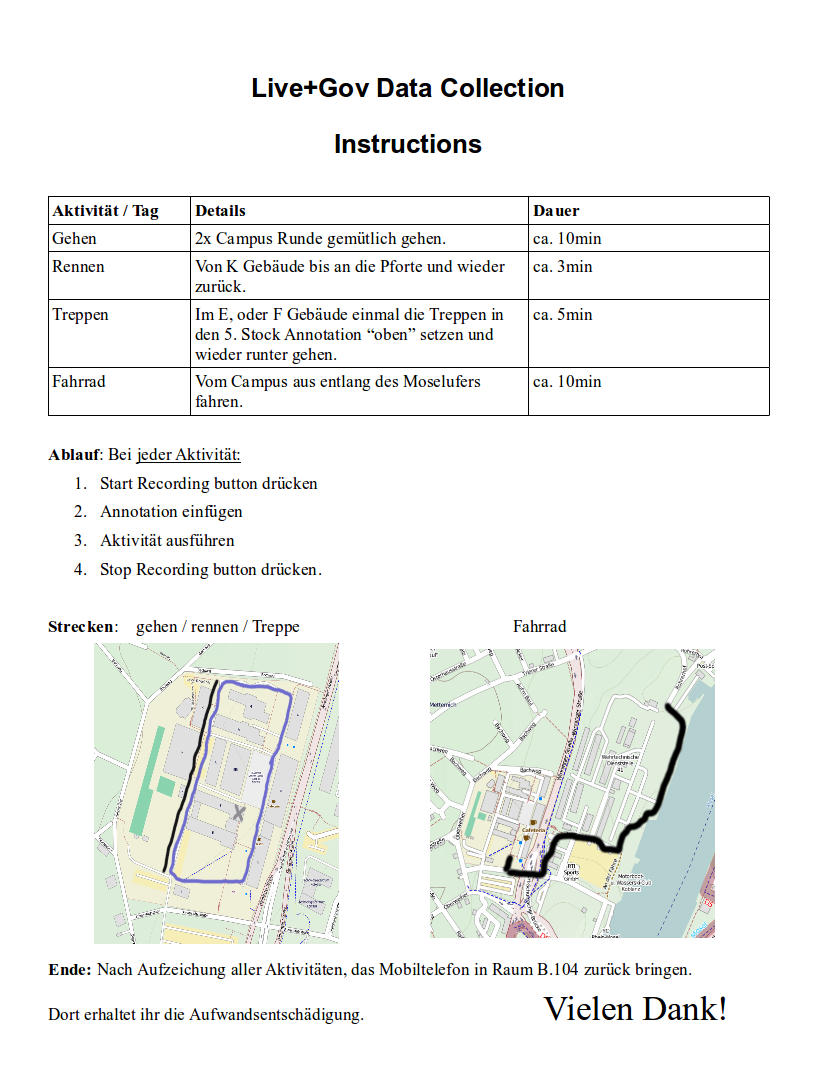
\includegraphics[width=\textwidth]{img/har/data_collection_handout.png}
%   \caption{Instructions for data collection in German
%     language}\label{fig:data_collection_handout}
% \end{figure}

The other dataset was obtained from the {\it UCI Machine Learning
  Repository}\footnote{\url{http://archive.ics.uci.edu/ml/datasets/Human+Activity+Recognition+Using+Smartphones}}
and was gathered by Davide Anguita, et. al. \cite{Anguita} in 2012.
It contains around $700K$ collected by 30 volunteers.

The number of samples per activity of both datasets are summarized in
Table \ref{fig:har_datasets}. Both datasets contain only
accelerometer samples, and have been preprocessed that have been
sampled at a fixed rate of $50Hz$.

\begin{table}[h]
\centering
\begin{tabular}{|l|r|r|} \hline
Activity  & UCI Dataset & UKOB Dataset \\ \hline
sitting   & 113.728     & 80.951        \\
standing  & 121.984     & 320.737       \\
walking   & 110.208     & 292.024       \\
running   & 0           & 31.916        \\
cycling   & 0           & 436.106       \\
stairs    & 188.800     & 30.086        \\
lying     & 124.416     & 0            \\ \hline \hline
Totals    & 659.136     & 903.156       \\ \hline
\end{tabular}
\caption{Number of accelerometer samples by activity and dataset.}
\label{fig:har_datasets}
\end{table}

Both datasets have been split into a training data-set and a test
data-set. The individual parts contain only full recordings of the
activities. No single recording is present in both parts of the
split. The volume is distributed in roughly $66/33$ ratio between
both parts.

We have three different parameters for the evaluation:
\begin{itemize}
\item {\bf Classifier.} Decision Tree (DT) or support vector machine (SVM)
\item {\bf Features.} Manually selected (MAN) or PCA based (PCA)
\item {\bf Dataset.} Self collected (UKOB) ore reference dataset (UCI)
\end{itemize}

We get the following evaluation results:
\begin{center}
\begin{tabular}{|lll|r|} \hline
  {\bf Classifier} & {\bf Features} & {\bf Dataset} & {\bf Accuracy in \%} \\ \hline
  DT	& MAN	& UKOB	&	$62$ \\ 
  DT	& PCA	& UKOB	&	$45$\\ 
  SVM	& MAN	& UKOB	& 	$\mathbf{87}$\\ 
  SVM	& PCA	& UKOB	&	$54$\\
  DT	& MAN	& UCI	&	$83$ \\ 
  DT	& PCA	& UCI	&	$68$ \\ 
  SVM	& MAN	& UCI	& 	$\mathbf{ 85 }$ \\ 
  SVM	& PCA	& UCI	&	$64$ \\ \hline
\end{tabular}
\end{center}

Figure \ref{fig:har_eval} shows a plot of these accuracy values.
\begin{figure}[ht]
  \centering
  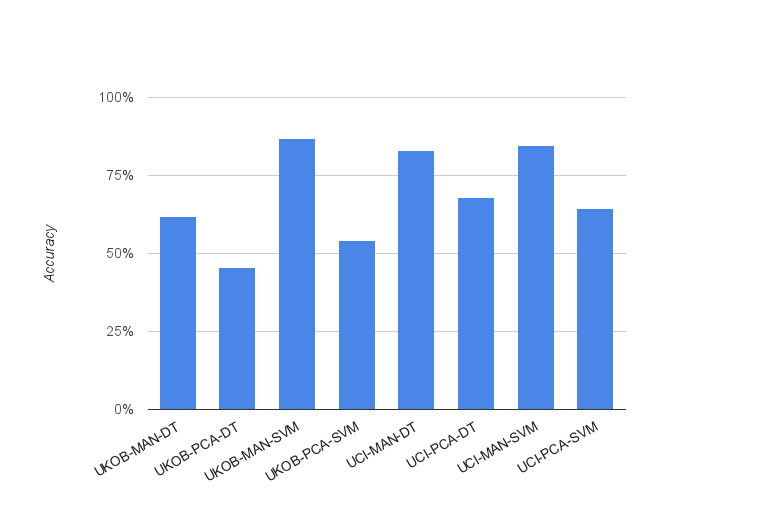
\includegraphics[width= 0.6 \textwidth]{img/har/accuracy_plot.png}
  \caption{Classification accuracy of HAR classifiers}
  \label{fig:har_eval}
\end{figure}

These figures show, that we are still around 10\% away from the state
of the art classifier used by \cite{Anguita} with 97\% accuracy. There
the authors use a multi-modal SVM on a similar list manually selected
feature vectors and slightly parameters for window length and overlap.
Our integrated application relies on a decision tree and manual
features, which show significantly weaker performance (64\%) than
state of the art in our experiments.

For both datasets the SVM trained on manual features performes best.
Although there are several parameters in the PCA feature extraction,
that remain to be optimized, the evaluation results suggest that
manually selected features yield better results.  For the UCI dataset
the decision tree is only slightly worse than the SVM based classifier
whereas the UKob dataset shows a more significant drop of
accuracy. This might be due to the fact that UKob dataset contains
slightly different activities than UCI, e.g. a large number samples is
recorded for the cycling activity, which is not present at UCI, and
conversely no samples for the lying task are present.

% Another anomaly is visible in the confusion matrices (cf. section
% \ref{sec:confusion_matrices}), is that we were not able to recognize
% the activity ``sitting'' in our own dataset. We do not currently have
% a good explanation of this anomaly. It points to structural problems
% in our approach, that need to be investigated further.

In conclusion, we have presented here a working HAR classification
architecture, that has been fully integrated into a mobile device and
has been evaluated against state of the art classifiers from the
literature on different datasets. Although the classification
accuracies are still behind state of the art, we are confident that we
can improve our methods exploiting the built up infrastructure.

% \clearpage
% \subsubsection{\bf Confusion Matrices}
% \label{sec:confusion_matrices}
% UCI-MAN-DT

\begin{tabular}{|l|rrrrrr|} \hline
Activitites & laying & sitting & stainding & walking & stairs down & stairs up\\
\hline
laying & 664 & 0 & 0 & 0 & 0 & 0\\
sitting & 0 & 542 & 64 & 0 & 0 & 0\\
standing & 0 & 135 & 521 & 0 & 0 & 0\\
walking & 0 & 0 & 0 & 1468 & 162 & 101\\
stairs down & 0 & 0 & 0 & 294 & 205 & 41\\
stairs up & 0 & 0 & 0 & 193 & 21 & 273\\
\hline
\end{tabular}

UKOB-MAN-DT

\begin{tabular}{|l|rrrrr|} \hline
Activities & cycling & running & sitting & stairs & walking\\
\hline
cycling & 1290 & 3 & 0 & 2 & 184\\
running & 0 & 30 & 0 & 0 & 29\\
sitting & 0 & 0 & 0 & 0 & 21\\
stairs & 15 & 0 & 1 & 92 & 127\\
walking & 142 & 11 & 0 & 812 & 784\\
\hline
\end{tabular}

UCI-PCA-DT

\begin{tabular}{|l|rrrr|} \hline
Activities & laying & sitting & standing & walking\\
\hline
laying & 664 & 0 & 0 & 0\\
sitting & 22 & 519 & 28 & 37\\
standing & 0 & 126 & 512 & 18\\
walking & 0 & 25 & 21 & 1685\\
\hline
\end{tabular}

UKOB-PCA-DT

\begin{tabular}{|l|rrrrr|} \hline
 & cycling & running & sitting & stairs & walking\\
\hline
cycling & 1051 & 64 & 1 & 1 & 362\\
running & 14 & 2 & 0 & 0 & 43\\
sitting & 747 & 0 & 0 & 0 & 32\\
stairs & 0 & 33 & 0 & 80 & 122\\
walking & 6 & 729 & 0 & 80 & 122\\
\hline
\end{tabular}

UKOB-MAN-SVM

\begin{tabular}{|l|rrrrr|} \hline
activities & cycling & running & sitting & stairs & walking\\
\hline
cycling & 1289 & 1 & 11 & 16 & 147\\
running & 0 & 59 & 0 & 0 & 0\\
sitting & 0 & 0 & 0 & 21 & 0\\
stairs & 12 & 0 & 0 & 75 & 140\\
walking & 57 & 0 & 1 & 60 & 1631\\
\hline
\end{tabular}

UCI-MAN-SVM

\begin{tabular}{|l|rrrrrr|} \hline
 & laying & sitting & standing & walking & stairs down & stairs up\\
\hline
laying & 664 & 0 & 0 & 0 & 0 & 0\\
sitting & 12 & 547 & 47 & 0 & 0 & 0\\
standing & 0 & 61 & 595 & 0 & 0 & 0\\
walking & 0 & 0 & 0 & 1642 & 71 & 18\\
stairs down & 0 & 3 & 0 & 291 & 230 & 16\\
stairs up & 0 & 0 & 0 & 185 & 15 & 287\\
\hline
\end{tabular}

UKOB-PCA-SVM

\begin{tabular}{|l|rrrrr|} \hline
 & cycling & running & sitting & stairs & walking\\
\hline
cycling & 1020 & 4 & 64 & 1 & 390\\
running & 38 & 0 & 0 & 0 & 21\\
sitting & 0 & 0 & 779 & 0 & 0\\
stairs & 203 & 1 & 0 & 3 & 28\\
walking & 1206 & 5 & 0 & 12 & 526\\
\hline
\end{tabular}

UCI-PCA-SVM

\begin{tabular}{|l|rrrrrr|} \hline
 & laying & sitting & standing & walking & stairs down & stairs up\\
\hline
laying & 664 & 0 & 0 & 0 & 0 & 0\\
sitting & 9 & 535 & 49 & 13 & 0 & 0\\
standing & 0 & 155 & 500 & 1 & 0 & 0\\
walking & 25 & 12 & 322 & 1307 & 32 & 33\\
stairs down & 21 & 2 & 79 & 432 & 5 & 1\\
stairs up & 6 & 1 & 31 & 432 & 7 & 10\\
\hline
\end{tabular}


%%% Local Variables:
%%% mode: latex
%%% TeX-master: "../D1-2"
%%% End:



%%% Local Variables:
%%% mode: latex
%%% TeX-master: "../D1-2"
%%% End:


\section{Service Line Detection}

One part of the user contextualization is the service line detection. The aim of this component is to recognize if a citizen uses public transport within the HSL area in Helsinki. If such a usage is detected, the right service line id with its direction and the further itinerary will be determined. Based on this information it is possible to solve higher level tasks like traffic jam detection, connecting train recommendation, or network utilization analysis.

The service line detection is implemented as a server side mining component which provides a REST API for answering user queries in real time. For long term evaluations all API calls are recorded and send to the L+G Service Center on a daily bases. Due to the seamless integration into the L+G ecosystem, where each user gets an universal unique id, all received tracks are personalized and can be combined with additional information coming from other components. In a later analysis, the service line detection results can be augmented with the low level human activity recognition data of the same user to gain a better insight into the users behavior.

\begin{figure}[ht]
\centering
\subfigure[]{
  \frame{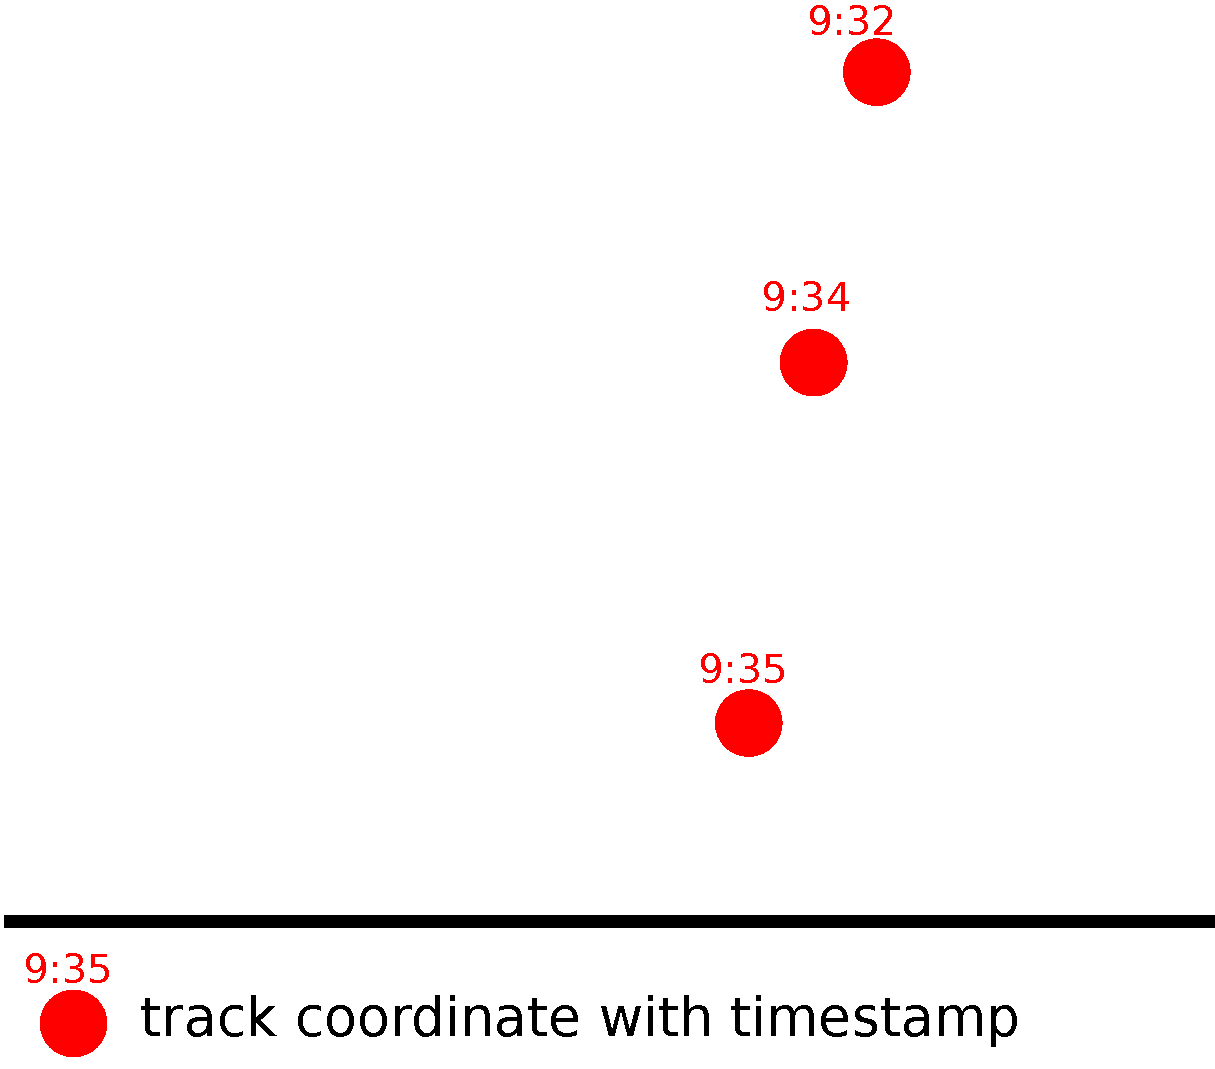
\includegraphics[width=0.3\textwidth,natwidth=556.19,natheight=432]{img/SLD/track.pdf}}
  \label{fig:track}
  \setcounter{subfigure}{1}
} 
\subfigure[]{
  \frame{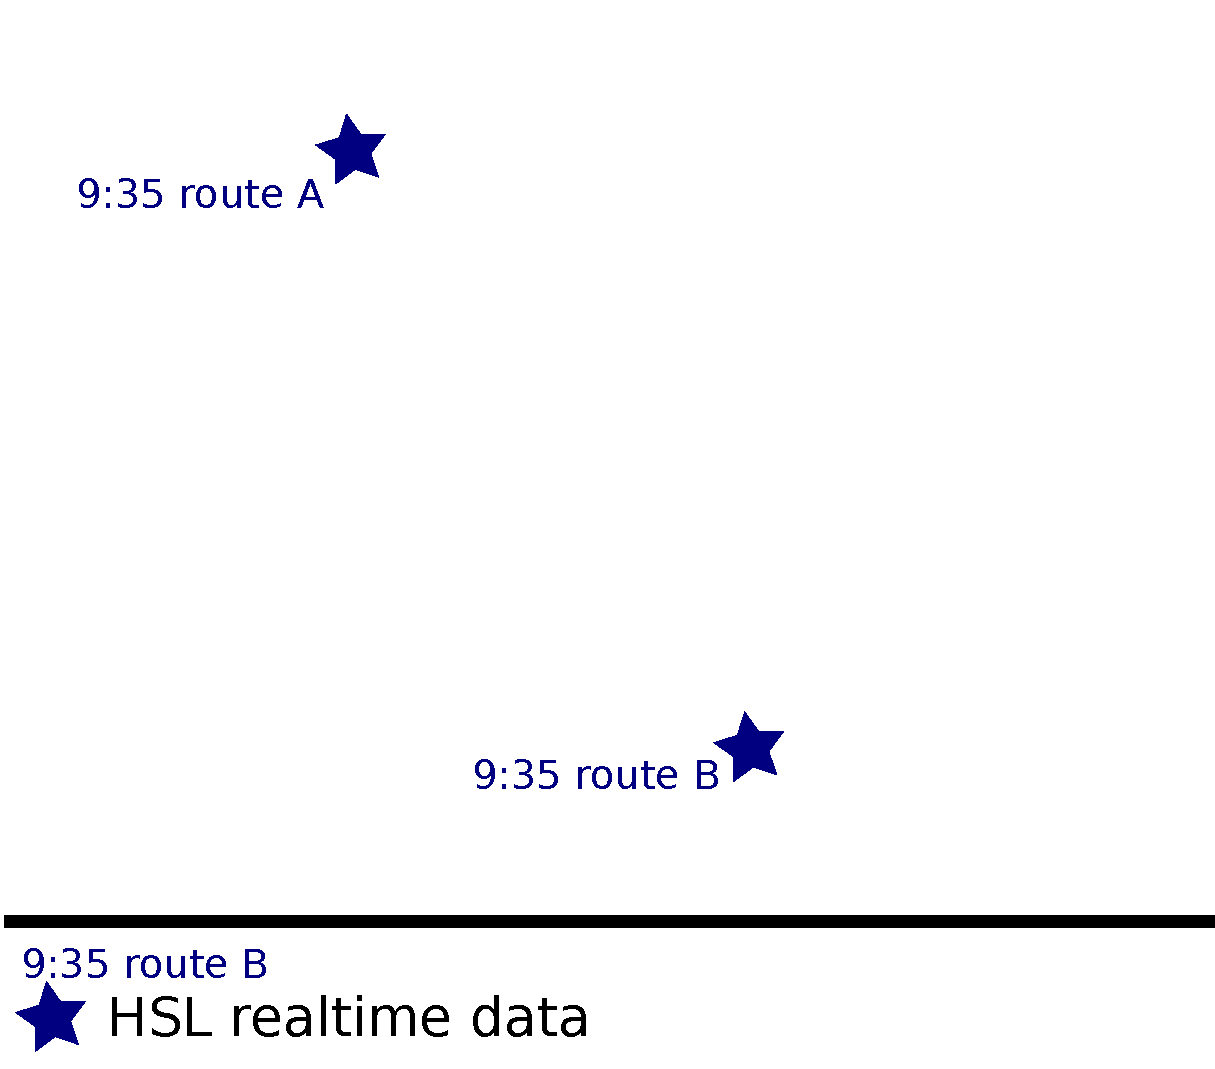
\includegraphics[width=0.3\textwidth,natwidth=556.19,natheight=432]{img/SLD/realtime.pdf}}
  \label{fig:realtime}
  \setcounter{subfigure}{2}
}
\subfigure[]{
  \frame{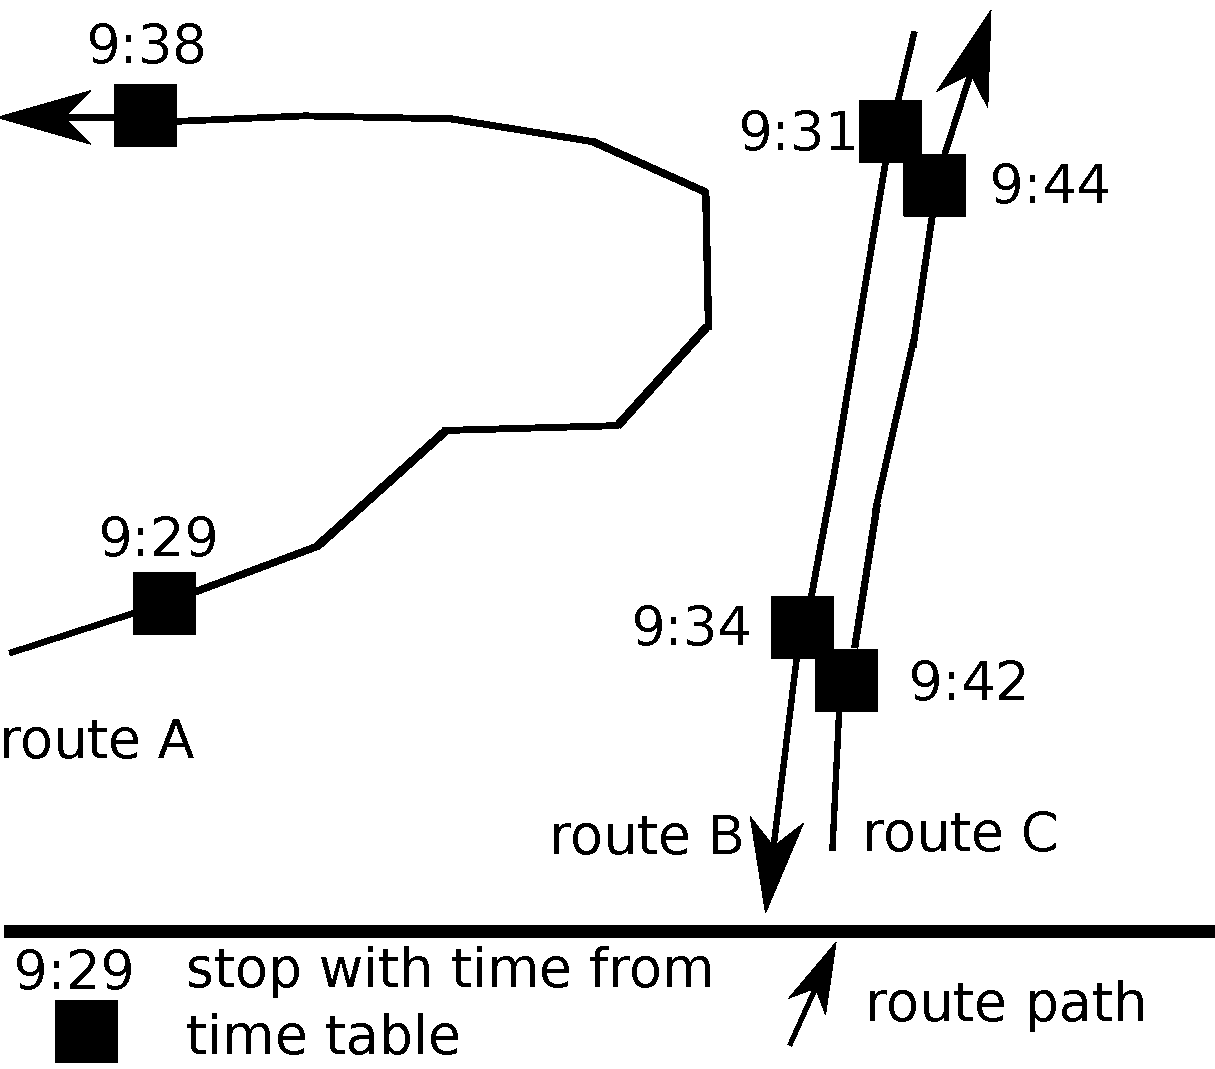
\includegraphics[width=0.3\textwidth,natwidth=556.19,natheight=432]{img/SLD/static.pdf}}
  \label{fig:static}
  \setcounter{subfigure}{3}
}
\subfigure[]{
  \frame{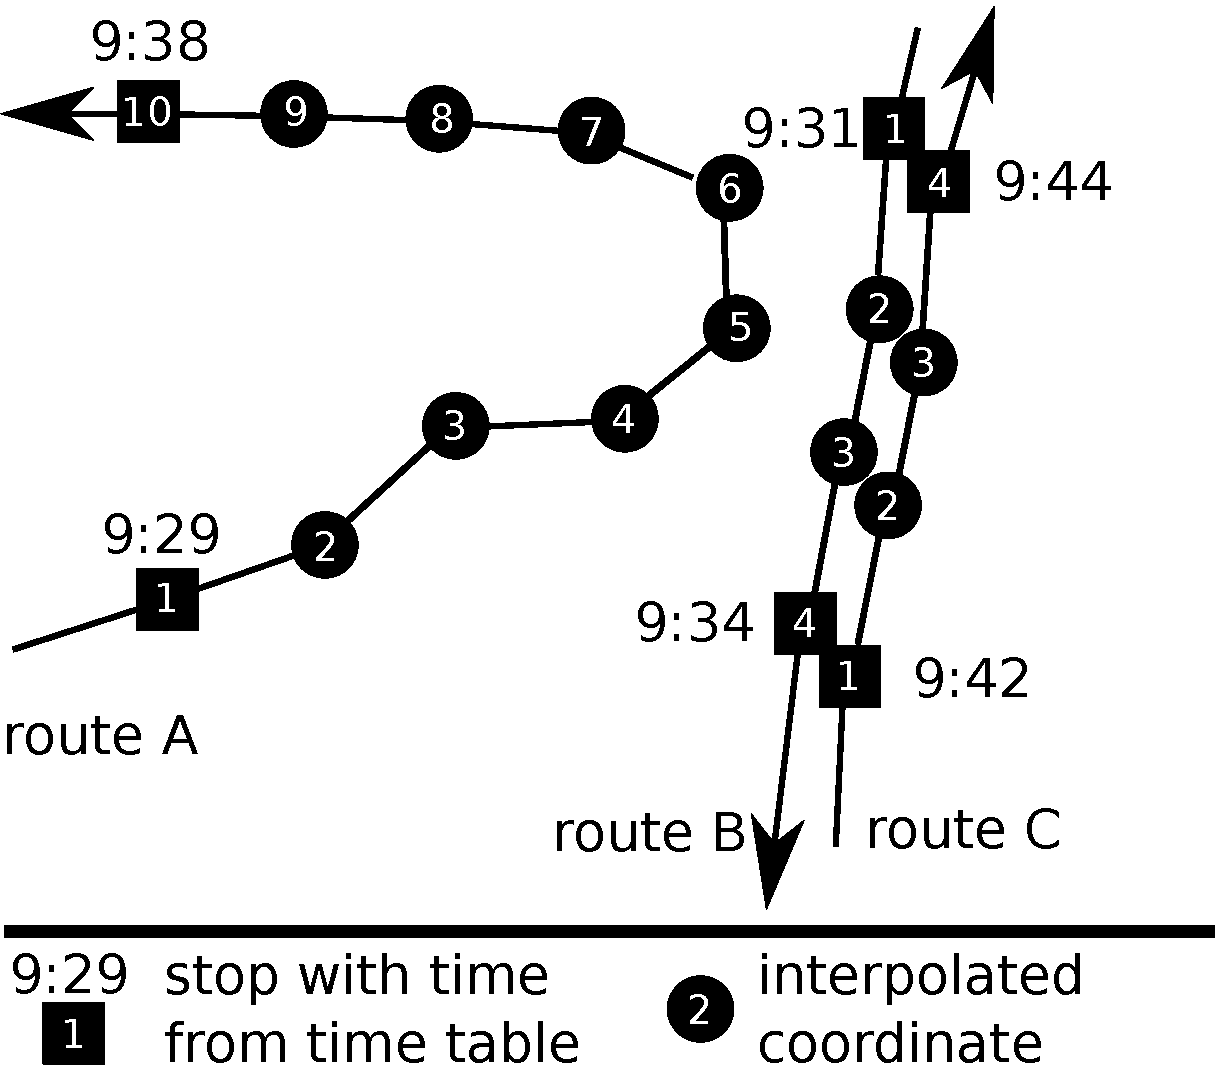
\includegraphics[width=0.3\textwidth,natwidth=556.19,natheight=432]{img/SLD/interpolatedCoords.pdf}}
  \label{fig:interpolatedCoords}
  \setcounter{subfigure}{4}
}
\subfigure[]{
  \frame{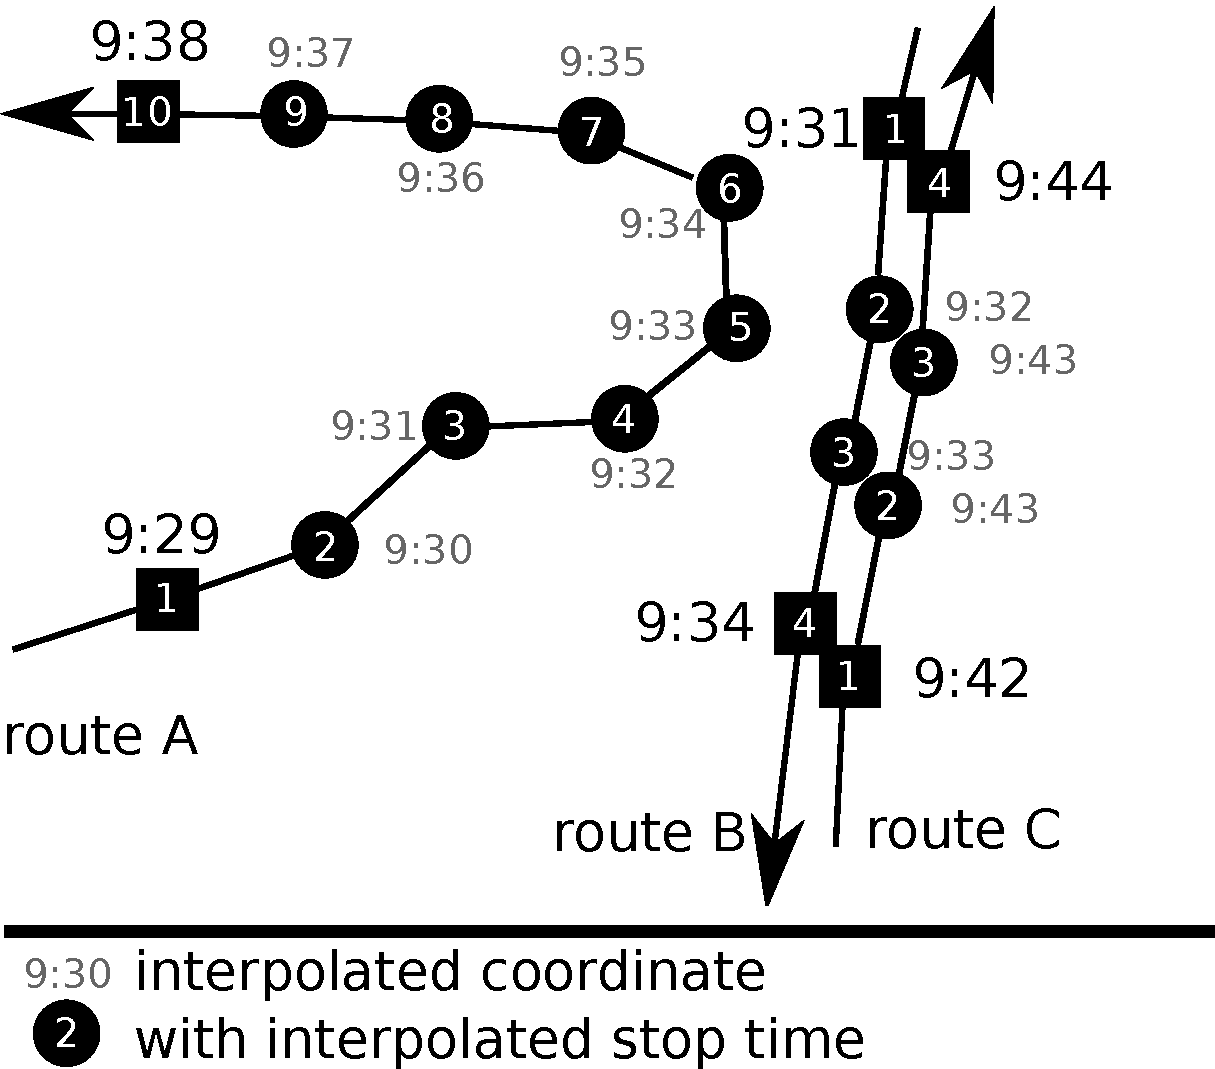
\includegraphics[width=0.3\textwidth,natwidth=556.19,natheight=432]{img/SLD/interpolatedCoordsWithTimes.pdf}}
  \label{fig:interpolatedCoordsWithTimes}
  \setcounter{subfigure}{5}
} 
\subfigure[]{
  \frame{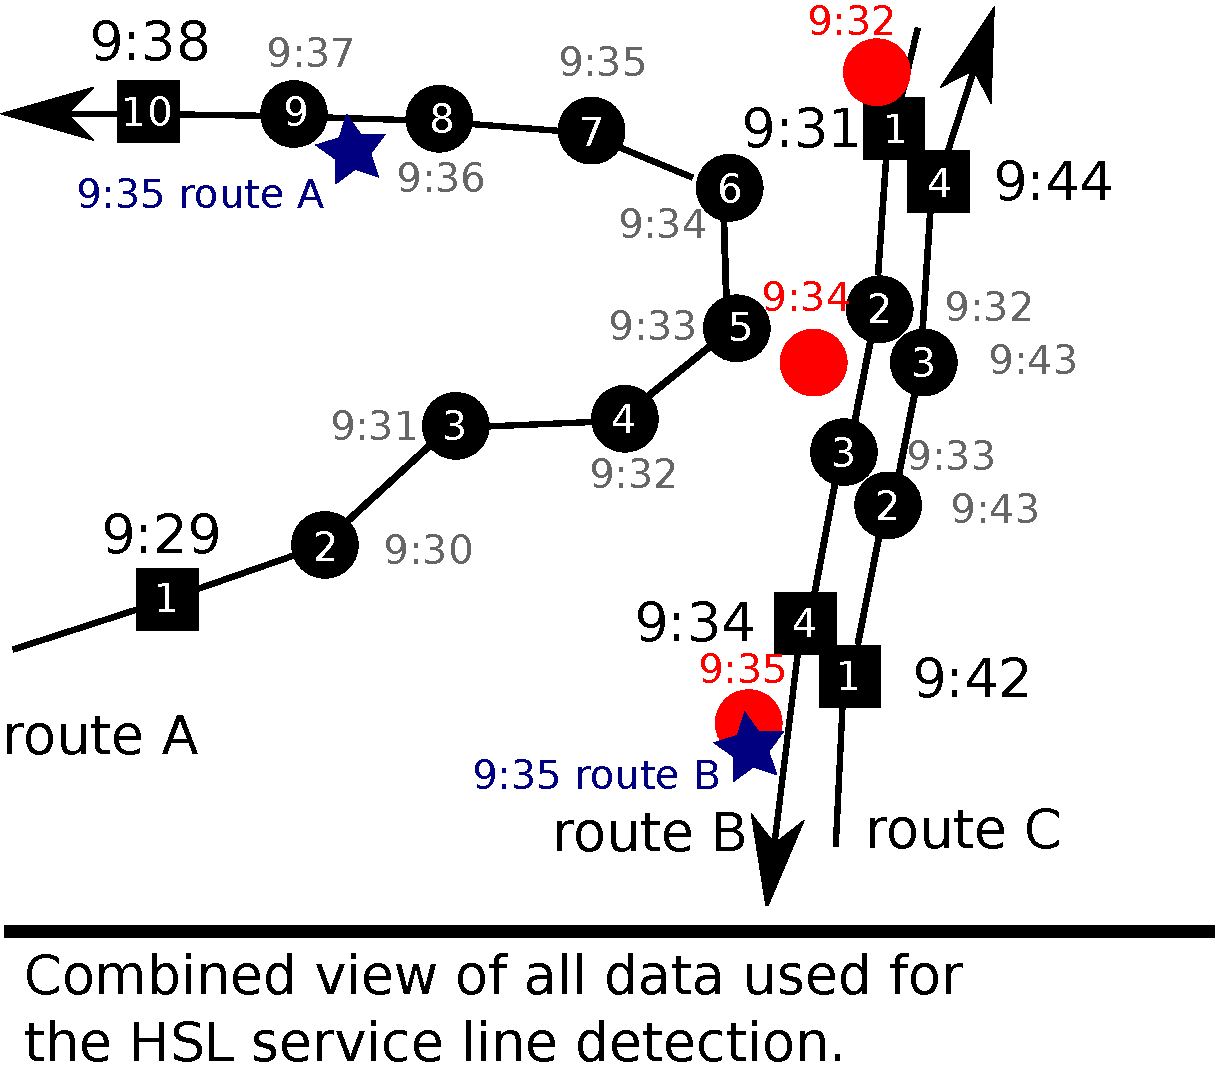
\includegraphics[width=0.3\textwidth,natwidth=556.19,natheight=432]{img/SLD/combined.pdf}}
  \label{fig:combined}
  \setcounter{subfigure}{6}
}
\caption{
The various input data for the HSL service line detection.
}
\label{fig:SLD}
\end{figure}

Assigning a trajectory to a specific service line requires the access to suitable background knowledge. In the Helsinki case it is two fold:
First of all, the system is fed with all HSL public transportation schedules and associated geographic information of stops and travel paths. By means of this dataset the theoretical position of every vehicle at any point in time can be calculated. A drawback of only including static time tables is that actual schedule deviations stay disregarded. This gap is closed by the HSL Live API, which is the second data source the service line detection relies on. With this API, the actual positions of some vehicles can be determined. Especially trams are tracked in realtime and can be accessed via this interface.  Unfortunately, the vast majority of vehicles, such as buses, have not yet been integrated. Lacking a complete realtime coverage is why still some uncertainty remains in the overall system. Therefore, the main challenge is to combine both kinds of data to archive the best possible performance.

Just as the background data, the classification algorithm is also two-stage. Given an user trajectory containing a small set of GPS coordinates with timestamps (Figure~\ref{fig:track}), in a first step the algorithm checks if the latest given timestamp is near the actual time. If so, the HSL Live API is called in order to find all vehicles which are currently around the user (Figure~\ref{fig:realtime}). Service lines found below a certain distance to the user are scored with a high probability to be the true line belonging to the given track.

In a second step, each coordinate of the given track is compared to the static route data (Figure~\ref{fig:static}) obtained from the time tables and paths.
It should be noted that the public transportation schedules only contain exact arrival times for each stop, but don't provide any time data for the pathes between them. Since this data is too sparse to perform reliable service line detection on it, all paths are rasterized evenly (Figure~\ref{fig:interpolatedCoords}) and the corresponding time for each intermediate part is interpolated (Figure~\ref{fig:interpolatedCoordsWithTimes}). This ensures that no route section falls through the cracks when executing a simple distance query in time and space. Figure~\ref{fig:combined} shows the combined view of all data used for the HSL service line detection.

The result of the algorithm is the one service line which has the highest probability due to the Live API and/or the smallest distance to the given set of coordinates. During a testing phase, the optimal values of all involved parameters like distance thresholds, time and space raster sizes, and the individual scoring weights have to be learned. As one outcome of the Helsinki field trial, we expect to find a good heuristic how to setup the various ingredients of the algorithm.

\subsection{Implementation details}
As a starting point, HSL provided us with all static service line data like arrival times, stop positions, route meta data, and path files in the well known General Transit Feed Specification (GTFS)\footnote{\url{https://developers.google.com/transit/gtfs/}} format. The original data set had a size of 400 MB and was imported into a PostgreSQL database. All paths and stop positions were stored as native geospatial values using PostGIS, a spatial database extender for PostgreSQL. After the import, we found 587 distinct routes, 7534 stops, and a total number of 206,153 trips in the database. In general, a service line like the bus 934 from Myyrm\"{a}ki to Luhtaanm\"{a}ki, has two directions, travels along its route path and stops at its stops. If a service line runs every ten minutes, each trip has its own trip id and is uniquely identifiable.

While these data are too sparse for distance queries, we interpolate the possible positions of a vehicle along its path to ensure that the distance between two consecutive trip positions is always smaller than ten meter. On the one hand, this simplifies a query like "find all trips in a distance of 20 meters around the user which arrive in plus minus one minute from now" a lot. On the other hand, the interpolation and denormalization inflates the data. Resulting in 324,440,457 trip positions annotated with arrival time and trip id, we enlarged the original data to a size of 38 GB.

This size leads the PostGIS index to its limit and prevents response times below 30 seconds for a service line detection query. Therefore, all data was partitionated horizontally in time dimension. The reason is, that all time tables repeat itself every 7 days and an usual query covers only a very small period of time at a specific weekday. Against this background, we divided the data into 24 parts for every day, which results in 7 times 24 subtables in the database. Finally, this setting archives average response times of less than one second for a whole service line detection query, containing of up to 200 single distance queries.


\subsection{Evaluation}
How did we test the quality of the classifier.

\section{Traffic Jam Detection}
\todo{MTS}{Add content.}

\subsection{Related Work}
Explain common approaches to Traffic Jam detection or related problems.

\subsection{Component Description}
Explain implementation. 

\subsection{Evaluation}
How was the quality of the jam detection classifier assessed?

\section{Distributed Geo-Matching}
\todo{DJ}{Add content.}
%--------------------------------------------------------------------
%\chapter{Example Section}
%--------------------------------------------------------------------

%%% Local Variables: 
%%% mode: latex
%%% TeX-master: "../D1-2"
%%% End: 

%\subsection*{Geographical Data and Social Media}

Nowadays, the means of public transportation become equipped with physical sensors like GPS sensors or light barriers. Those sensors are used to keep track of the current vehicle position or to estimate the number of passengers. But those sensors do not detect, for instance, emergencies, accidents or the passengers' opinions on bus lines. To overcame these limitations, another kind of sensors is required.

In the last decade, many social networks or micro-blogging services like Twitter\texttrademark arose. They are frequently used by humans to publish their opinions, observations, etc. which then can be requested by a web API. Therefore, the users of those services can be seen as social sensors. The increasing number of mobile phones leads to a situation in which more and more passengers become social sensors by publishing statements about crowded buses or rioting passengers.

The evaluation of the social sensor data requires that the bus or train can be identified to which a message is related. This task is simplified by the fact that most mobile phones have integrated GPS sensors. They measure the current geographical position, which is added to the published message together with a timestamp. This position information can be used to identify the nearest train or bus. A more detailed description of this matching problem  will be given in the next section.

The amount of data produced by the different types of sensors can exceed the processing capabilities of a single computer. Therefore, a distributed approach is required, which will be explained in section \ref{sec:approach}. Finally, the results of an experiment with the current implementation are presented in section \ref{sec:experiment}.

\subsection{Problem of Matching Physical and Social Sensor Data}\label{sec:problem}

In order to find the bus or train a message is related to, the data measured by the physical sensors have to be processed first. In this context, the relevant data consists of the longitude and latitude measured by the GPS sensors of the vehicles. Before transmitting these data, they have to be extended by the unique id of the current vehicle and a timestamp to keep track of the chronological order. The set of all possible position is defined as $Pos$ in equation (\ref{eqn:Pos}).

\vspace*{-2\baselineskip}
\begin{eqnarray}
 Pos & := & V_{id} \times T \times \mathbb{R} \times \mathbb{R}\label{eqn:Pos}
\end{eqnarray}

The relevant data of the social sensors are the messages published by the passengers. Each message contains a timestamp, i.e., the publishing time and the GPS position of the mobile phone from which the message was sent. The set of all possible messages $Mes$ is defined in equation (\ref{eqn:Mes}) where $C$ is the set of all possible message contents.

\vspace*{-2\baselineskip}
\begin{eqnarray}
 Mes & := & T \times \mathbb{R} \times \mathbb{R} \times C\label{eqn:Mes}
\end{eqnarray}

The data of the different sensors are transmitted as a not necessarily finite stream of data as defined in the equations (\ref{eqn:posStream}) and (\ref{eqn:mesStream}).

\vspace*{-2\baselineskip}
\begin{eqnarray}
 posStream: &  & \mathbb{N} \rightarrow Pos\label{eqn:posStream}\\
 mesStream: &  & \mathbb{N} \rightarrow Mes\label{eqn:mesStream}
\end{eqnarray}

The range of $posStream$, i.e., the set of vehicle position received by the data stream $posStream$ are the trajectories of the different vehicles. A trajectory is defined in equation (\ref{eqn:traj}) as a discrete function mapping some point in time to a geographical position.

\vspace*{-2\baselineskip}
\begin{eqnarray}
 traj: & & T \mapsto \mathbb{R} \times \mathbb{R}\label{eqn:traj}
\end{eqnarray}

But this definition is not adequate because the timestamps of messages may vary from the timestamps contained in the position data of the vehicles. Therefore, a continuous trajectory function $\widehat{tray}$ is required. This is reached by, for instance, a linear interpolation of $tray$.

Equation (\ref{eqn:allTraj}) shows the function $allTraj$ which maps the unique identifier of a vehicle on its corresponding continuous trajectory.

\vspace*{-2\baselineskip}
\begin{eqnarray}
 allTraj: & & V_{id} \mapsto (T \mapsto \mathbb{R} \times \mathbb{R})\label{eqn:allTraj}
\end{eqnarray}

In order to relate a message $m$ to a bus or train, the vehicle must be determined which has the smallest euclidean distance $dist$ to the position of the sender at the point in time when $m$ was sent. Furthermore, a vehicle has a maximum length $maxDist$ and all vehicles with a greater distance from $m$ can be ignored. Thus, each message can be seen as a range nearest-neighbour query $rnn$ as defined in equation (\ref{eqn:rnn}).

\vspace*{-2\baselineskip}
\begin{eqnarray}
 &&rnn: Mes \rightarrow Pos \cup \{\texttt{null}\} \textrm{ with}\label{eqn:rnn}\\
 &&rnn((t,lon_m,lat_m,cont)):= (vId,t,lon_v,lat_v)\nonumber\\
 &&\hspace*{1cm}\textrm{if } allTraj(vId)(t)=(lon_v,lat_v) \wedge dist((lon_m,lat_m),(lon_v,lat_v))\leq maxDist \wedge \nonumber\\
 &&\hspace*{1cm}\not\exists vId' \in V_{id}: dist((lon_m,lat_m),allTraj(vId')(t))< dist((lon_m,lat_m),allTraj(vId)(t))\nonumber\\
 &&rnn((t,lon_m,lat_m,cont)):= \texttt{null}\nonumber\\
 &&\hspace*{1cm}\textrm{otherwise}\nonumber
\end{eqnarray}

Putting it all together, the problem of finding the nearest vehicle for each message is defined as followed:

{
\definecolor{mygray}{gray}{.75}
\fbox{\colorbox{mygray}{\parbox{\columnwidth}{
\textbf{Problem} Finding range nearest vehicle for each message\\
\textbf{Input:} $posStream$, $mesStream$, $maxDist$\\
\textbf{Output:} $rnnStream: \mathbb{N} \rightarrow Mes \times Pos \bullet rnnStream(i):=(mesStream(i),rnn(mesStream(i)))$
}}}
}

An implementation which solves this problem has to deal with the fact, that the data received by different sensors are not equally delayed. For instance, the data measured from physical sensors may be faster transmitted then messages received from social networks.

Another difficulty is, that the amount of data received by the different input streams may exceed the processing capabilities of a single computer. One solution for this problem would be to discard incoming data if the load of the single machine would be to high. This could lead to the loss of valuable data. In order to avoid this, a distributed approach is required which scales horizontally.

Some approaches like PLACE* \cite{Xiong2007PAD} distribute the incoming data according to a static mapping of computers on geographical regions. The disadvantage of this static mapping can be seen, for instance, if there exists a sport stadium in some region. If a sport event takes place, then there are many vehicles and passengers producing a huge amount of data. Therefore, the corresponding computer can only deal with a relatively small region. But if not event takes places, this computer does nearly have no work. In order to improve this, the mapping has to be dynamic, i.e., a dynamic load balancing is required.

\subsection{Distributed Geo-Matching Approach}\label{sec:approach}

The schema of an intuitive stream-processing system which solves the problem described above can be seen in figure \ref{subfig:localRtree}. It consists of a single component ($C$) which receives the incoming data streams of vehicle positions and messages. It caches the current positions and processes the range nearest-neighbour queries initiated by the received messages. The answers are transmitted via the outgoing data stream $rnnStream$.

In order to answer range nearest-neighbour queries, $C$ has to cache the current position of all vehicles. The problem of the delayed sensor data requires the caching of more vehicle positions than just the latest. Thus, a sliding window approach is implemented with a window size exceeding all regular delay times. This is realized by deleting all vehicle positions outside the window whenever a new position with a timestamp later then the timestamp of the latest cached position is received.

The data structure used as cache should answer range nearest-neighbour queries efficiently. In spatio-temporal databases R*-trees \cite{Beckmann1990TRA} are used for this purpose. Similar to a B-tree, the inserted elements are stored only in the leafs. Each node except the root has a minimal and a maximal number of children or elements. If an insertion is performed on a node already containing the maximal number of elements, then it is split and the resulting inner node is inserted in the parent node. In contrast to B-trees, each node of an R*-tree represents the minimal bounding rectangle (MBR) of all elements contained in its subtree as illustrated in figure \ref{fig:Rtree}. The presented tree consists of a root node (dark gray), seven leafs (light gray) and several vehicle positions (black squares).

\begin{figure}[htbp]
\centering
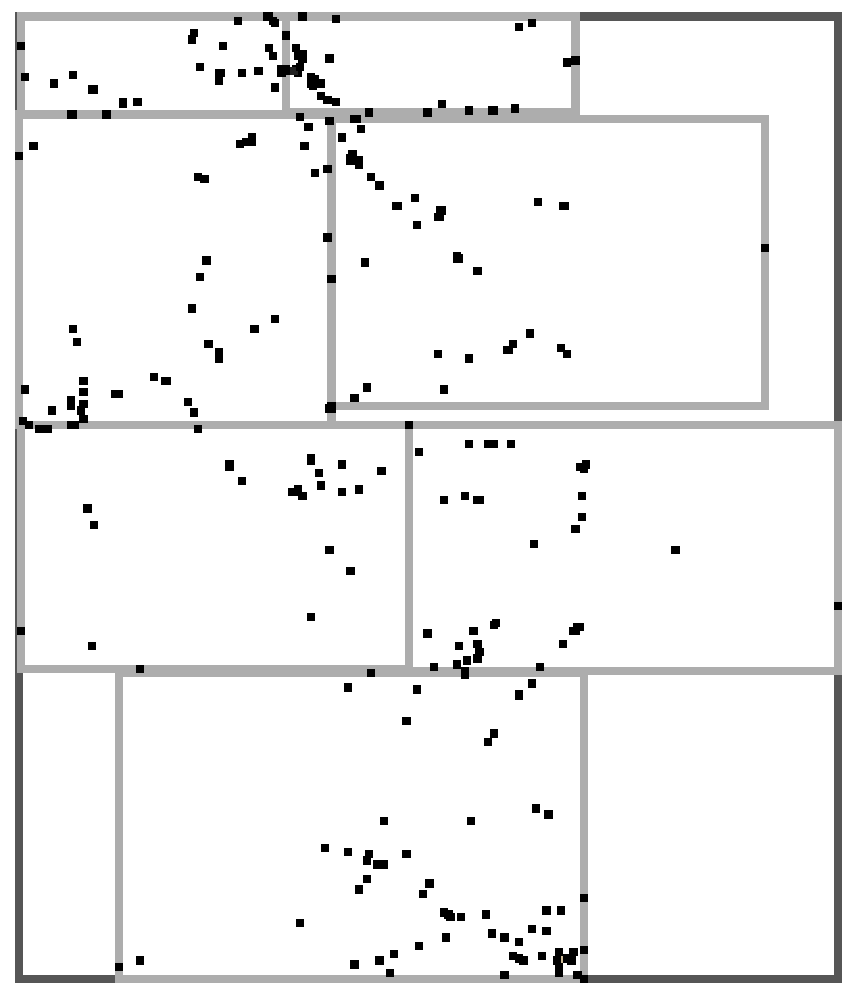
\includegraphics[scale=0.3,angle=90]{img/dgm/rTree.pdf}
\caption{An examplary R*-tree}\label{fig:Rtree}
\end{figure}

During the processing of a range nearest-neighbour query, only the children of a node are visited whose MBR intersects with the queried range. Thus, the performance of the query processing depends on the number of subtrees to be traversed. In order to reduce this number, the MBRs of the child nodes should be disjoint. As shown in \cite{Beckmann1990TRA} the algorithms used for insertion and deletion are designed to ensure a minimal overlap of MBRs. Another advantage is, that the MBRs are dynamically adjusted according to the currently contained elements.

\begin{figure}[htbp]
\centering
\subfigure[A system with a single cache]{
\label{subfig:localRtree}
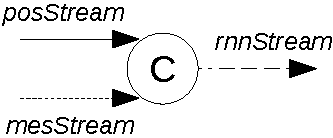
\includegraphics[scale=0.6]{img/dgm/SingleCache.pdf} 
}
\subfigure[A system with several caches]{
\label{subfig:rootRtree}
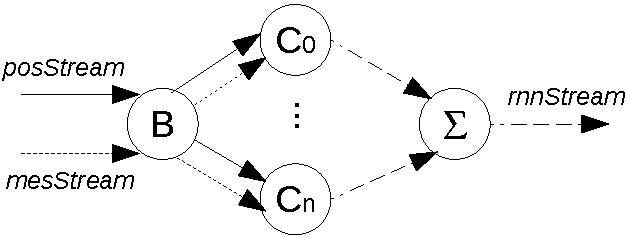
\includegraphics[scale=0.6]{img/dgm/MultiCache.pdf} 
}
\subfigure[A distributed R*-tree]{
\label{subfig:distributedRtree}
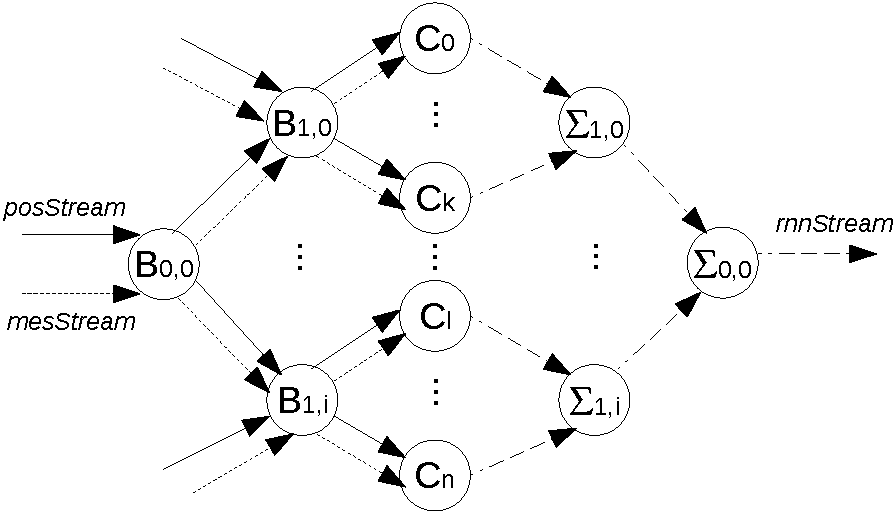
\includegraphics[scale=0.6]{img/dgm/DistributedTree.pdf} 
}
\caption{Distributing a geo-matching system}\label{fig:DistributedRtree}
\end{figure}

The problem of the system shown in figure \ref{subfig:localRtree} is that its processing capabilities are quite limited. Therefore, a distributed approach is required which spreads the load on several computers. Figure \ref{subfig:rootRtree} shows such a system. It consists of several caches $C_0$ to $C_n$ each of them owning an own R*-tree for caching current vehicle positions and responding to queries.

Furthermore, this system consists of balancer component $B$. It receives the incoming streams of vehicle positions and messages and decides to which of the different caches each single datum is sent. Similar to the root of an R*-tree, it keeps track of the MBRs of the different caches. A new vehicle position is basically sent to the cache with the nearest MBR. If $B$ receives a new message, it is only forwarded to the caches whose MBR intersects with the queried range. In the best case this is only one cache. But it could be several caches as well. Thus a special combiner component ($\Sigma$) is required which receives the nearest vehicle of each cache involved inte the query processing and returns the overall nearest neighbour.

A further responsibility of $B$ is the load balancing, i.e., the number of cached vehicle positions and queries in progress should be similar for all caches. Therefore, $B$ counts the number of vehicle positions and messages forwarded to the different caches. The load balancing is done by distributing the received vehicle positions according to special target ranges for the different caches. In the case of a balances system, these regions are equal to the MBRs. But if the load of a cache $C_i$ exceeds the load of a cache $C_j$ with a neighboured MBR, than the target range of $C_i$ is reduced and the range of $C_j$ increased. During the progress of the sliding window the MBRs of the caches will approach their target ranges.

In regular intervals, $B$ sends special requests to all caches to send the information about their current loads and MBRs back (not shown in figure \ref{subfig:rootRtree}). If $B$ receives the responses of all caches, it updates its calculated values. These update requests are performed asynchronously, i.e., the distribution of the incoming data is not blocked. This leads to a situation that the information received by the caches are not up to date any more. Therefore, $B$ caches all forwarding decisions from the time the updated request is sent until all caches have responded. Then these decisions are applied on the received load information and MBRs.

The disadvantage of this system is, that the single balancer component $B$ and combiner component $\Sigma$ can become bottlenecks. A future solution could be found when thinking of $B$ as the root of distributed R*-tree whose children are the trees stored in the different caches. If it is close to its processing limits, it creates child balancer components which are responsible for subregions of the overall MBR. Each of the children gets an input stream for all the data of its MBR. Data for regions which are not covered by the children are still received by the root. Whenever a balancer component is split the combiner components are split analogously. Such a system is illustrated in figure \ref{subfig:distributedRtree}.

\subsection{Experiment}\label{sec:experiment}


\section{Geographic Topic Analysis}
%--------------------------------------------------------------------
%\chapter{Topic Models}
%--------------------------------------------------------------------

The BuitenBeter dataset consists of 13,811 geo-tagged issues reported to the
office of public order in the Netherlands between July and September 2012.  Each
issue is assigned to one of 16 categories such as "poor road conditions", "Dirt
on the street" or "Graffiti".

Geographical co-occurrences of arbitrary categorical observations - such as
public order issues of the BuitenBeter dataset - can be used to discover latent
underlying factors that explain observations which co-occur more frequently than
expected by chance.  One method for detecting these latent factors is
probabilistic topic modelling, where grouped observations are modelled as being
sampled from mixtures of latent topics, which are probability distributions over
the set of distinct observations.

For the BuitenBeter dataset, we e.g. might expect that areas where graffities
are reported will see many reports of the category "Dirt on the street" since
both categories are related to urban environments. We model those environments
as hidden "topics".
  
Existing approaches for geographical topic modelling adopt topic models such as
latent Dirichlet allocation \cite{Blei:2003:LDA:944919.944937} and extend the
models by assigning distributions over locations to topics, or by introducing
latent geographical regions. In models which extend topics for spatial
distributions (such as two-dimensional normal distributions)
\cite{conf/wsdm/Sizov10}, topics with a complex (i.e. non-Gaussian) spatial
distribution cannot be detected. In models with latent, Gaussian distributed
regions \cite{conf/www/YinCHZH11}, documents within a complex shaped topic area
do not influence the topic distribution of distant documents within the same
area. Therefore, topics with a complex spatial distribution such as topics
distributed along coastlines, rivers or country borders are harder to detect by
such methods.  More elaborate models introduce artificial assumptions about the
structure of geographical distributions, e.g. by introducing hierarchical
structures \cite{ahmed13} in advance.
%Additionally, some approaches \cite{conf/www/MeiLSZ06,conf/www/YinCHZH11} do not model document-specific
%topic distributions. 

We introduce a novel geographical topic model which captures dependencies
between geographical regions to support the detection of topics with complex,
e.g. non-Gaus\-sian distributed spatial structures \cite{CCK1}.
%The model is based on a hierarchical Dirichlet process
%extended to support multiple base distributions, which we name MDP. 
%Our method thus is called the MDP-based geographical topic model (MGTM). 
%We use the MDP to dynamically smooth topic distributions between groups of spatially
%adjacent documents.

Our model differs from existing approaches in several aspects:

We model locations and words separately, as the separation of spatial clusters
and document semantics allows us to define meaningful neighbour relations
between spatially adjacent clusters. Our topic model takes a set of geographical
clusters as input.

We also expect that geographical clusters adjacent in space exhibit similar
topic distributions: Most geographical topics cannot be approximated by a simple
spatial probability distribution such as a Gaussian distribution and for these
complex topic areas, coherent sets of multiple spatial distributions are a
reasonable approximation.  Therefore we detect and smooth the topic distribution
of these adjacent regions to increase the probability of detecting coherent
topic areas.

The detection of geographical clusters is straight-forward: We use a mixture of
a fixed number of Fisher distributions -- distributions on a three dimensional
unit sphere similar to isotropic Gaussian distributions on a plane. The
parameters are fit using the approximation given by Banerjee et
al.~\cite{DBLP:journals/jmlr/BanerjeeDGS05} in an expectation-maximisation
algorithm.  In our model, each cluster is associated with a distribution over
the set of topics, sampled from a Dirichlet process (DP) with a common base
measure which is itself drawn from a DP with Dirichlet distributed multinomial
distributions over the set of categories as base measure.  For the smoothing of
topic distributions of adjacent clusters, we first define the adjacency relation
using the Delaunay triangulation \cite{journals/csur/Aurenhammer91} of the
cluster centroids.  Each public order issue report draws an own topic
distribution from a DP with a weighted mixture of the topic distribution of its
own geographical cluster and its neighbour clusters as base measure.  Finally,
each observed report category is drawn from its document-specific topic
distribution.  For a detailed description of the model and its parameters, we
refer to our paper \cite{CCK1}.

To train our model on the BuitenBeter dataset, we use 300 clusters and the
initial settings for the parameters $\beta = 0.5$, $\gamma = 1.0$, $\alpha_0 =
1.0$, $A = 99999$, $\delta = 1.0$. By setting $A$ to such a high value, we give
up document-specific topic distributions and sample the categories directly from
a mixture of region-specific topic distributions. All other parameters are set
to the values used in the paper \cite{CCK1}, except for the hyperparameters for
$A$, which is fixed.

For creating a comprehensible report, the detected topics can be characterised
by their most-likely categories:

Topic 1: \textit{Dirt on the street}, \ \textit{Other}, \ \textit{Graffities\\}
Topic 2: \textit{Damaged street light}, \ \textit{Bad road}\\
Topic 3: \textit{Obstacle by trees}, \ \textit{Weed}, \ \textit{Loose paving stones}, \ \textit{Bad road}, \ \textit{Idea/wish}\\
Topic 4: \textit{Other}, \ \textit{Weed}, \ \textit{Loose paving stones}, \ \textit{Bad road}, \ \textit{Damaged street light}, \ \textit{Idea/wish}


%for reduzing the size, set the width to 0.22\textwid
\begin{figure}[]
\centering
\subfigure[Topic 1]{
  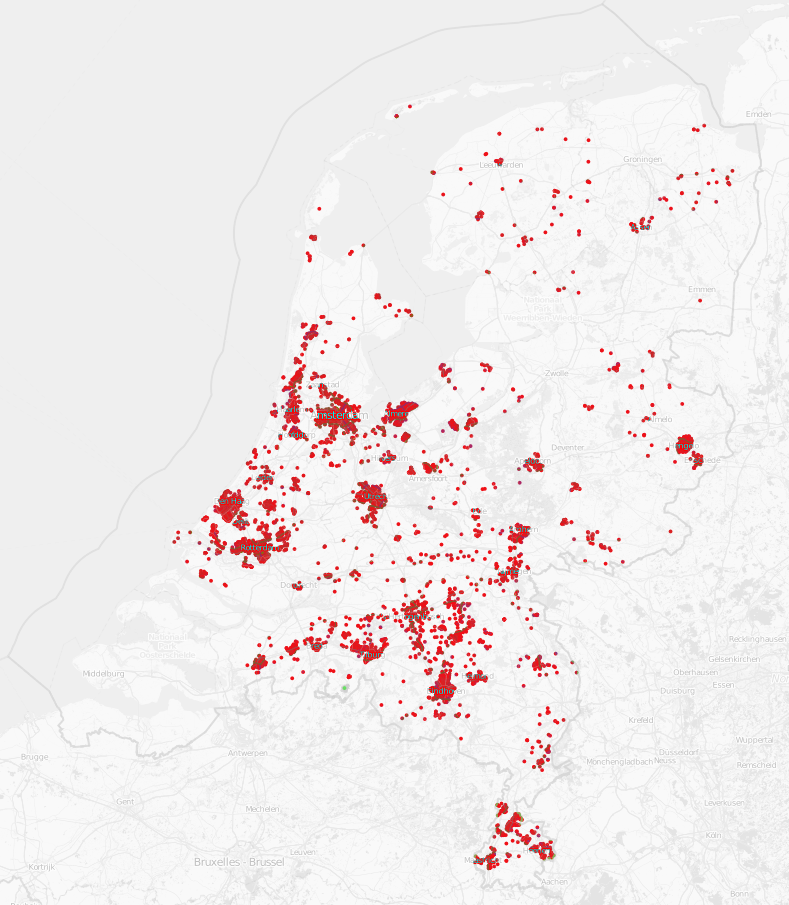
\includegraphics[width=0.3\textwidth,natwidth=556.19,natheight=432]{img/map/1.png}
  \label{plot:act20}
  \setcounter{subfigure}{1}
} 
\subfigure[Topic 2]{
  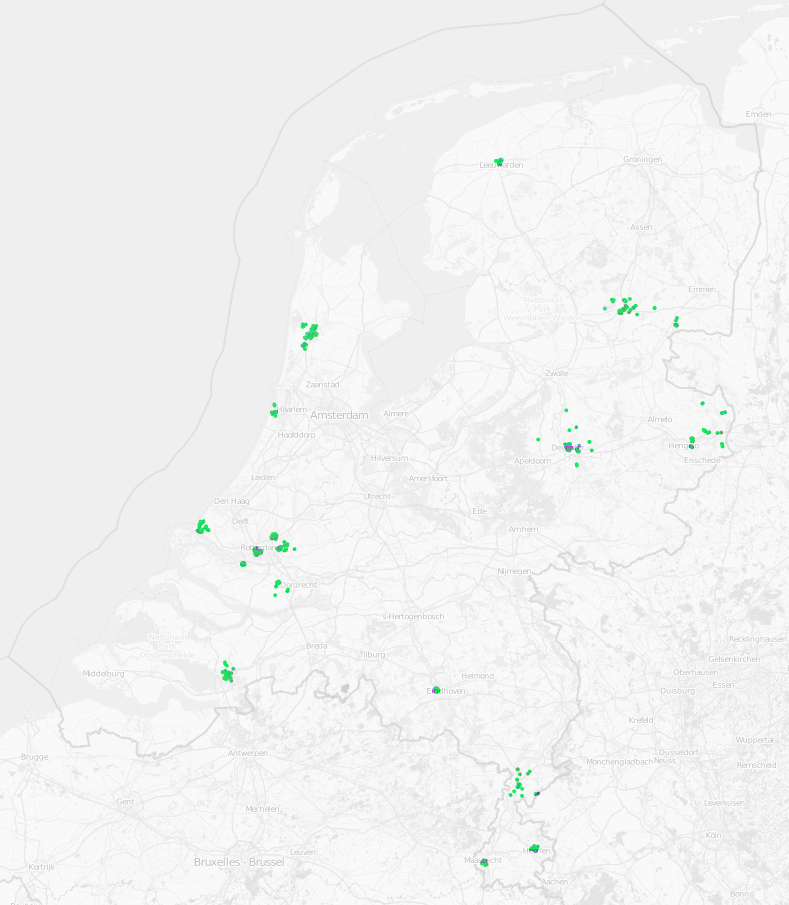
\includegraphics[width=0.3\textwidth,natwidth=556.19,natheight=432]{img/map/2.png}
  \label{plot:act20}
  \setcounter{subfigure}{2}
}

\subfigure[Topic 3]{
  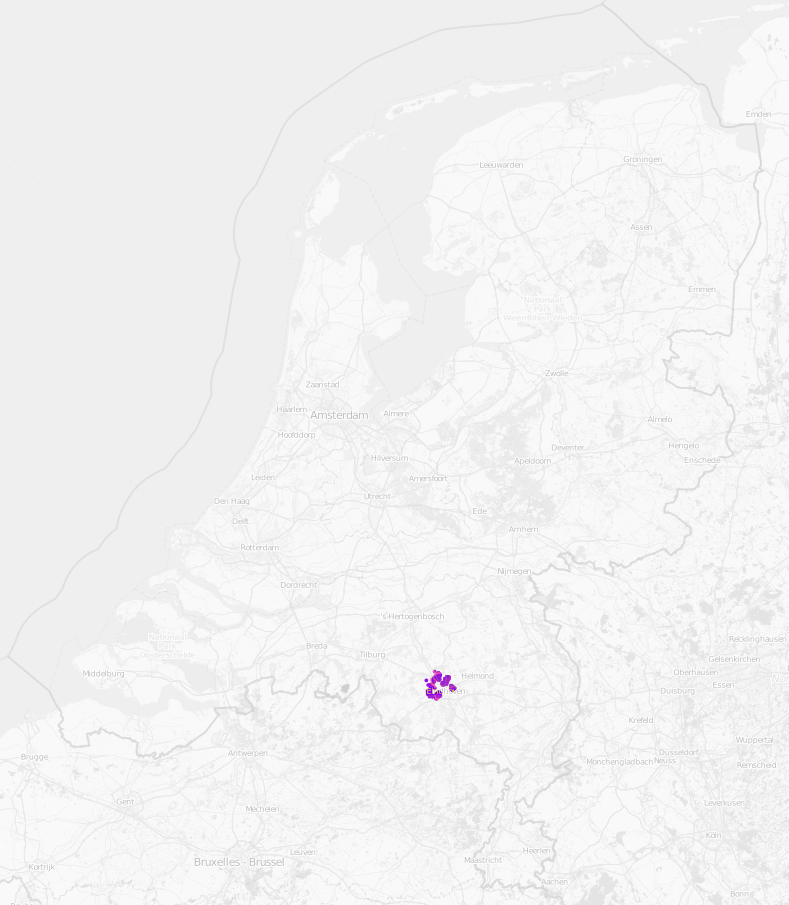
\includegraphics[width=0.3\textwidth,natwidth=556.19,natheight=432]{img/map/3.png}
  \label{plot:act20}
  \setcounter{subfigure}{3}
}
\subfigure[Topic 4]{
  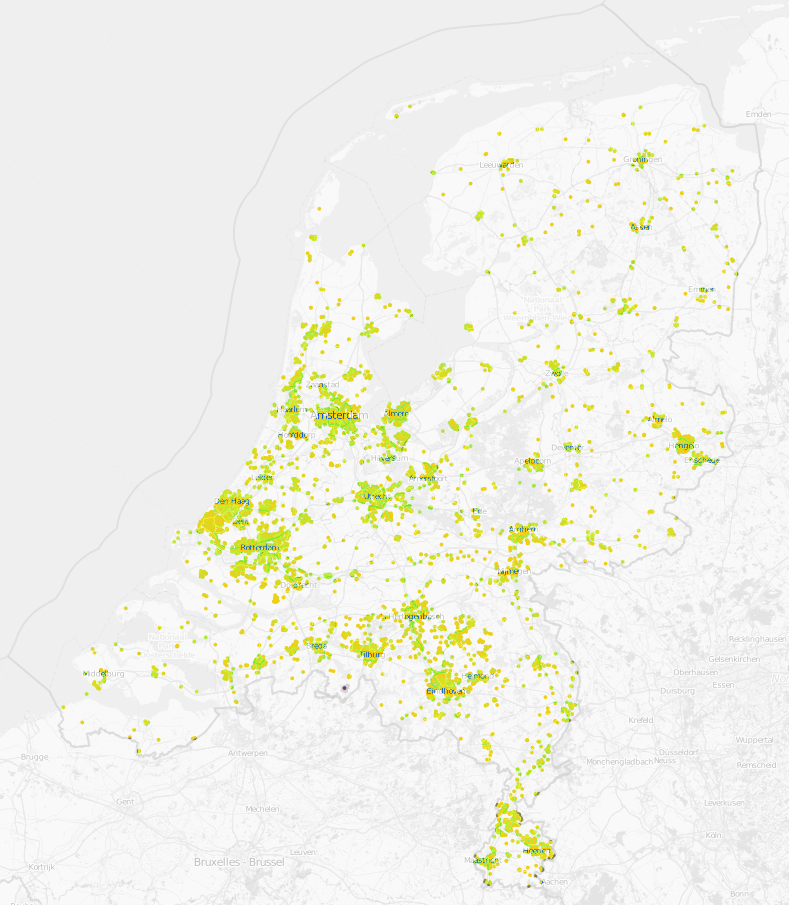
\includegraphics[width=0.3\textwidth,natwidth=556.19,natheight=432]{img/map/4.png}
  \label{plot:act20}
  \setcounter{subfigure}{4}
} 

\caption{
  Document positions of reports with above-average probabilities for Topic 1-4 on the map of the Netherlands.
}
\label{fig:netmaps}
\end{figure}

The position of documents with an above-average probability for each topic are
shown in \vbox{Figure \ref{fig:netmaps}}.  We see that, as expected, Topic 1 is
only observed in the area of larger cities, whilst Topic 4 is present across the
whole country.  Topic 2 occurs mostly within city centres.  Topic 3 is observed
in the area of Eindhoven for which different categories were available in the
BuitenBeter application.

%%% Local Variables: 
%%% mode: latex
%%% TeX-master: "../D1-2"
%%% End: 


\bibliography{D1-2}

\end{document}
